\documentclass[20pt, cjk, slidetop, table]{beamer}

\usepackage[UTF8]{ctex}
\usepackage{geometry}
\geometry{papersize={33cm,19cm},left=0.4cm,right=0.4cm}
\usepackage{amsmath,bm}
\usepackage{graphicx}
\usepackage{booktabs}
\usepackage{tabularx}
\usepackage{array}
\usepackage{ragged2e}
\usepackage{xcolor}
\usepackage{tikz}
\usetikzlibrary{arrows,positioning,fit,calc}
\usepackage{hyperref}
\usepackage{CQUPT}

\graphicspath{{figures/}{pic/}}
\hypersetup{colorlinks=false}
\setbeamertemplate{navigation symbols}{}
\setbeamertemplate{caption}[numbered]
\setbeamerfont{frametitle}{size=\Large}
\setbeamertemplate{itemize item}{\color{qut}$\blacktriangleright$}
\setbeamertemplate{itemize subitem}{\color{qut}$\bullet$}

\definecolor{cquptblue}{HTML}{00407A}
\definecolor{passgreen}{HTML}{12823B}
\definecolor{warnorange}{HTML}{C56A00}
\definecolor{softblue}{HTML}{EAF3FB}
\definecolor{softgreen}{HTML}{EAF7EF}
\definecolor{softorange}{HTML}{FFF1E3}
\definecolor{softgray}{HTML}{F4F6F8}
\definecolor{darkgray}{HTML}{333333}

\newcolumntype{Y}{>{\RaggedRight\arraybackslash}X}
\renewcommand{\arraystretch}{1.15}
\newcommand{\code}[1]{\texttt{\detokenize{#1}}}
\newcommand{\pass}{\textcolor{passgreen}{\textbf{达标}}}
\newcommand{\partialpass}{\textcolor{warnorange}{\textbf{ACLR 达标 / NMSE 未达标}}}
\newcommand{\metric}[3]{%
  \begin{beamercolorbox}[wd=\linewidth,sep=0.55em]{#1}%
    {\large\textbf{#2}}\par{\footnotesize #3}%
  \end{beamercolorbox}}

\setbeamercolor{metricpass}{fg=passgreen,bg=softgreen}
\setbeamercolor{metricwarn}{fg=warnorange,bg=softorange}
\setbeamercolor{metricblue}{fg=cquptblue,bg=softblue}
\setbeamercolor{card}{fg=darkgray,bg=softgray}

\title[轻量级 AI DPD 结题答辩]{轻量级 AI DPD 算法结题答辩}
\subtitle{第三届华为无线“声光电磁”硬件创新竞赛 09 赛题}
\author[从容应队]{队伍：从容应队}
\institute[SCIE, CQUPT]{重庆邮电大学 通信与信息工程学院}
\date{2026年7月}

\begin{document}

\begin{frame}
  \titlepage
  \vspace{-0.6cm}
  \begin{center}
    
\includegraphics[width=0.13\linewidth]{pic/LogoCQUPT.jpg}

    \vspace{0.25cm}
    {\large 轻量、可解释、可部署的宽带 PA 数字预失真方案}
  \end{center}
\end{frame}

\begin{frame}{目录}
  \tableofcontents
\end{frame}

\section{团队信息}
\begin{frame}{队伍与分工}
  \begin{columns}[T,onlytextwidth]
    \begin{column}{0.56\linewidth}
      \begin{tabularx}{\linewidth}{c c c Y}
        \toprule
        姓名 & 年级 & 学院 & 主要分工 \\
        \midrule
        XXX & XXX & 通信与信息工程学院 & 队长；算法设计与总体协调 \\
        XXX & XXX & 通信与信息工程学院 & 模型训练与消融实验 \\
        XXX & XXX & 通信与信息工程学院 & 指标评估与统一复现 \\
        XXX & XXX & 通信与信息工程学院 & 文档整理与答辩材料 \\
        \bottomrule
      \end{tabularx}
    \end{column}
    \begin{column}{0.38\linewidth}
      \begin{beamercolorbox}[wd=\linewidth,sep=0.9em]{metricblue}
        \textbf{基本信息占位}\par
        队长：XXX\par
        成员：XXX、XXX、XXX\par
        指导教师：XXX
      \end{beamercolorbox}

      \vspace{0.55cm}
      \begin{beamercolorbox}[wd=\linewidth,sep=0.9em]{card}
        \textbf{答辩关注点}\par
        DPD 任务理解、EA-TCN 方案、统一评估结果、低复杂度边界。
      \end{beamercolorbox}
    \end{column}
  \end{columns}
\end{frame}

\section{赛题与指标}
\begin{frame}{功放非线性使 DPD 成为必要前置补偿}
  \begin{columns}[T,onlytextwidth]
    \begin{column}{0.48\linewidth}
      \begin{itemize}
        \item 宽带 5G-A Pro 发射链路中，PA 同时存在 AM-AM、AM-PM 非线性。
        \item 记忆效应与残余群时延会让误差跨越多个采样点传播。
        \item 非线性谱再生直接抬高邻道泄漏，ACLR 成为硬约束。
        \item DPD 在数字基带侧学习 PA 逆系统，降低后端线性化压力。
      \end{itemize}
    \end{column}
    \begin{column}{0.48\linewidth}
      \begin{center}
        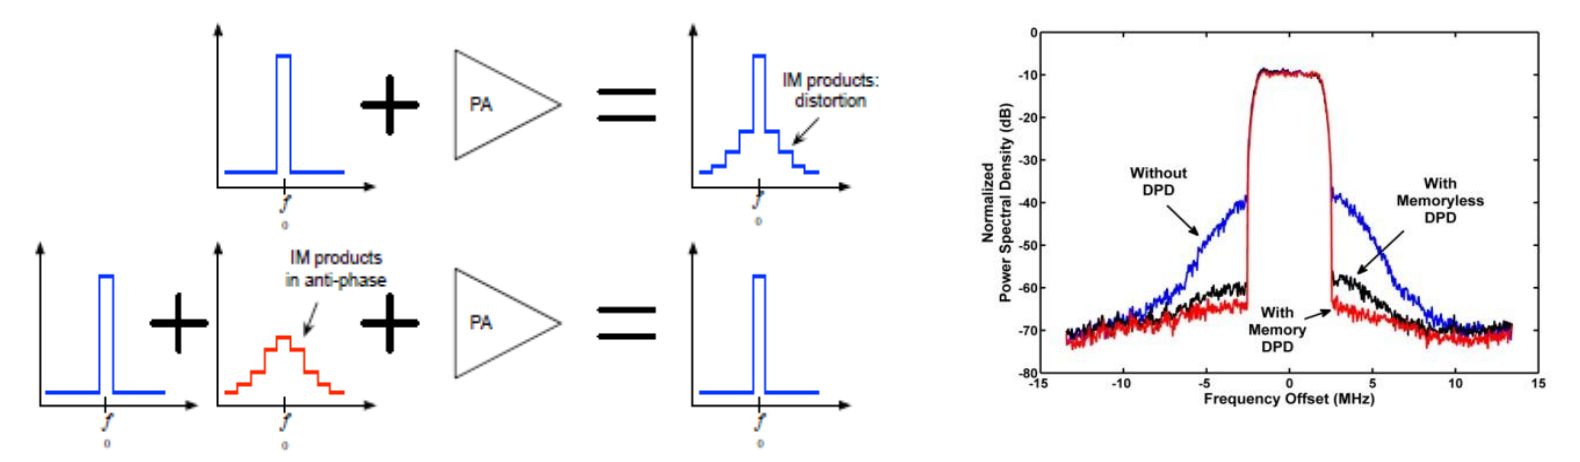
\includegraphics[width=0.9\linewidth]{figures/dpd_task.png}
      \end{center}
    \end{column}
  \end{columns}
\end{frame}

\begin{frame}{DPD 任务定义需要按时序验证}
  \begin{columns}[T,onlytextwidth]
    \begin{column}{0.54\linewidth}
      \begin{beamercolorbox}[wd=\linewidth,sep=0.9em]{metricblue}
        \textbf{学习目标}\par
        输入复数 IQ 序列 $x[n]$，模型输出 $\widehat{y}[n]=f_\theta(x)[n]$，使 \code{pred_y} 接近 \code{target_y}。
      \end{beamercolorbox}

      \vspace{0.45cm}
      \begin{itemize}
        \item 数据输入：复数 IQ 序列 $x[n]$。
        \item 切分方式：前 $80\%$ 训练，后 $20\%$ 验证。
        \item 切分原则：按时序切分，不打乱样本。
        \item 目的：避免宽带记忆系统的信息泄漏。
      \end{itemize}
    \end{column}
    \begin{column}{0.42\linewidth}
      \resizebox{\linewidth}{!}{%
      \begin{tikzpicture}[node distance=1.3cm,>=stealth,
        box/.style={draw=cquptblue,thick,rounded corners=2pt,fill=softblue,align=center,minimum height=1.15cm,minimum width=5.3cm},
        small/.style={draw=passgreen,thick,rounded corners=2pt,fill=softgreen,align=center,minimum height=1.05cm,minimum width=5.3cm}]
        \node[box] (x) {复数 IQ\\$x[n]=I[n]+jQ[n]$};
        \node[box,below=of x] (model) {DPD 模型\\$f_\theta(\cdot)$};
        \node[small,below=of model] (pred) {\code{pred_y}\\$\widehat{y}[n]$};
        \node[box,right=1.7cm of model] (target) {\code{target_y}\\目标线性响应};
        \draw[->,thick,cquptblue] (x) -- (model);
        \draw[->,thick,cquptblue] (model) -- (pred);
        \draw[->,thick,warnorange] (target) |- (pred);
        \node[align=center,below=0.8cm of pred] {\textcolor{darkgray}{以验证集 NMSE 与 ACLR 判定是否达标}};
      \end{tikzpicture}
      }
    \end{column}
  \end{columns}
\end{frame}

\begin{frame}{评价约束同时覆盖时域误差、邻道泄漏与 MAC}
  \begin{columns}[T,onlytextwidth]
    \begin{column}{0.58\linewidth}
      \begin{align*}
        \mathrm{NMSE} &=
        \frac{\sum_n |\widehat{y}[n]-y[n]|^2}{\sum_n |y[n]|^2},\\
        \mathrm{NMSE}_{\mathrm{dB}} &= 10\log_{10}(\mathrm{NMSE}),\\[0.35em]
        \mathrm{ACLR}_{\mathrm{dBc}} &=
        \operatorname{mean}(\mathrm{PSD}_{\mathrm{adjacent}})
        - \operatorname{mean}(\mathrm{PSD}_{\mathrm{main}}),\\
        \mathrm{ACLR}_{\mathrm{worst}} &=
        \max(\mathrm{ACLR}_{\mathrm{lower}},\mathrm{ACLR}_{\mathrm{upper}}).
      \end{align*}
    \end{column}
    \begin{column}{0.37\linewidth}
      \begin{tabularx}{\linewidth}{l Y}
        \toprule
        项目 & 口径 \\
        \midrule
        采样率 & 491.52 MHz \\
        主带 & $[-100,100]$ MHz \\
        下邻道 & $[-245,-180]$ MHz \\
        上邻道 & $[180,245]$ MHz \\
        达标目标 & NMSE $\le -40$ dB；worst ACLR $\le -45$ dBc \\
        复杂度 & 等效实数乘法器数 \\
        \bottomrule
      \end{tabularx}
    \end{column}
  \end{columns}
\end{frame}

\section{算法方案}
\begin{frame}{选择 TCN + FIR 是为了兼顾长记忆与部署}
  \begin{columns}[T,onlytextwidth]
    \begin{column}{0.54\linewidth}
      \begin{tabularx}{\linewidth}{l Y Y}
        \toprule
        路线 & 优点 & 局限 \\
        \midrule
        纯 CNN & 并行友好 & 感受野随层数线性增长 \\
        RNN/LSTM & 长依赖强 & 循环状态不利于高速流水 \\
        大模型 DNN & 拟合能力强 & MAC 与存储成本高 \\
        TCN + FIR & 并行、长记忆、DSP 友好 & 需控制主干容量与频域校正 \\
        \bottomrule
      \end{tabularx}
    \end{column}
    \begin{column}{0.4\linewidth}
      \begin{beamercolorbox}[wd=\linewidth,sep=0.85em]{metricblue}
        \textbf{本项目取舍}\par
        用扩张 TCN 负责非线性记忆，用复数 FIR 负责残余线性群时延和频谱翅膀。
      \end{beamercolorbox}

      \vspace{0.55cm}
      \begin{itemize}
        \item 推理过程无循环依赖。
        \item 卷积、逐点混合、FIR 均可硬件流水化。
        \item 复杂度可直接映射到 MAC 预算。
      \end{itemize}
    \end{column}
  \end{columns}
\end{frame}

\begin{frame}{EA-TCN 将物理先验、序列建模和频域校正串联}
  \small
  \begin{columns}[T,onlytextwidth]
    \begin{column}{0.56\linewidth}
      \begin{tikzpicture}[>=stealth,node distance=0.45cm,
        flowbox/.style={draw=cquptblue,thick,rounded corners=2pt,fill=softblue,align=center,minimum height=0.82cm,minimum width=4.7cm,font=\footnotesize},
        eval/.style={draw=passgreen,thick,rounded corners=2pt,fill=softgreen,align=center,minimum height=0.82cm,minimum width=4.7cm,font=\footnotesize}]
        \node[flowbox] (in) {Input-9 特征\\I/Q、时移、幅度幂次};
        \node[flowbox,below=of in] (tcn) {扩张 TCN 主干\\H15/L6, $[1,2,4,8,16,32]$};
        \node[flowbox,below=of tcn] (attn) {谱注意力门控\\幅度包络调节通道};
        \node[flowbox,below=of attn] (fir) {复数 FIR + LS refit\\43 taps};
        \node[eval,below=of fir] (out) {\code{pred_y} 与统一评估\\NMSE / ACLR / PSD / MAC};
        \draw[->,thick,cquptblue] (in) -- (tcn);
        \draw[->,thick,cquptblue] (tcn) -- (attn);
        \draw[->,thick,cquptblue] (attn) -- (fir);
        \draw[->,thick,cquptblue] (fir) -- (out);
      \end{tikzpicture}
    \end{column}
    \begin{column}{0.4\linewidth}
      \begin{center}
        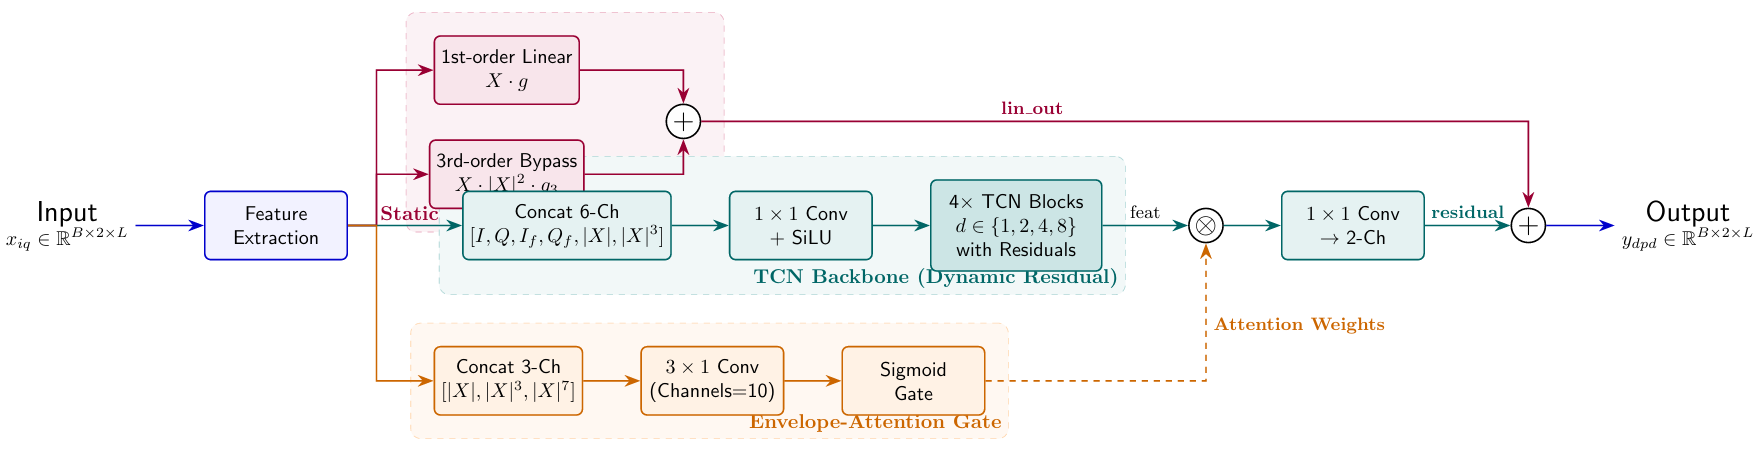
\includegraphics[width=0.86\linewidth]{figures/eatcn_template.png}
      \end{center}
      \begin{beamercolorbox}[wd=\linewidth,sep=0.45em]{card}
        \footnotesize
        四模块对应“特征先验、长记忆、幅度依赖、频域校正”，每一部分都能对应到 PA 线性化问题。
      \end{beamercolorbox}
    \end{column}
  \end{columns}
\end{frame}

\begin{frame}{Input-9 把低阶 PA 先验前置到特征侧}
  \begin{columns}[T,onlytextwidth]
    \begin{column}{0.47\linewidth}
      \begin{beamercolorbox}[wd=\linewidth,sep=0.9em]{metricblue}
        \textbf{Input-9 构成}\par
        I/Q、前后采样、幅度 $|x|$ 与高阶幅度特征，覆盖低阶 AM-AM / AM-PM 失真。
      \end{beamercolorbox}

      \vspace{0.55cm}
      \begin{itemize}
        \item 显式保留 $p=1,3,5$ 阶非线性基函数。
        \item 线性初始化吸收主缩放与相位旋转。
        \item 主干不必从零学习所有低阶物理先验。
      \end{itemize}
    \end{column}
    \begin{column}{0.49\linewidth}
      \begin{align*}
        x[n] &= I[n]+jQ[n],\\
        \phi_p(x[n]) &= x[n]\cdot |x[n]|^{p-1},\quad p\in\{1,3,5\},\\
        \mathbf{u}[n] &= \big[I,Q,I_{\pm1},Q_{\pm1}, |x|, |x|^3, |x|^5 \big].
      \end{align*}
      \begin{beamercolorbox}[wd=\linewidth,sep=0.7em]{card}
        特征增强的价值不是堆输入维度，而是把 PA 的幅度相关非线性显式暴露给轻量主干。
      \end{beamercolorbox}
    \end{column}
  \end{columns}
\end{frame}

\begin{frame}{扩张 TCN 用少量层覆盖长记忆}
  \begin{columns}[T,onlytextwidth]
    \begin{column}{0.45\linewidth}
      \begin{center}
        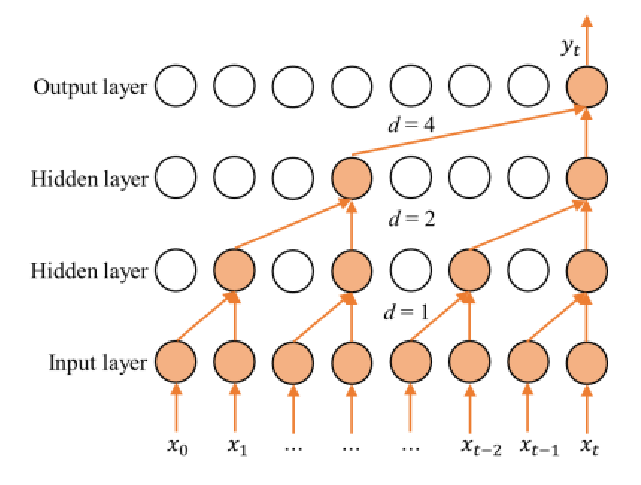
\includegraphics[width=0.92\linewidth]{figures/tcn_dilation.png}
      \end{center}
    \end{column}
    \begin{column}{0.5\linewidth}
      \begin{itemize}
        \item 主模型：H15/L6，dilations = $[1,2,4,8,16,32]$。
        \item 扩张卷积让感受野随层数近似指数增长。
        \item 对 $K=5$，主干感受野约为 $1+4(1+2+4+8+16+32)=253$ 个采样点。
        \item 并行卷积比循环结构更适合高速 DPD 推理。
      \end{itemize}
    \end{column}
  \end{columns}
\end{frame}

\begin{frame}{谱注意力按幅度区间调节通道响应}
  \begin{columns}[T,onlytextwidth]
    \begin{column}{0.5\linewidth}
      \begin{align*}
        \mathbf{a}[n] &= \big[|x[n]|,\ |x[n]|^3,\ |x[n]|^5\big],\\
        \mathbf{g}[n] &= \sigma\big(W_2\,\psi(W_1\mathbf{a}[n])\big),\\
        \widetilde{\mathbf{z}}[n] &= \mathbf{g}[n]\odot \mathbf{z}[n].
      \end{align*}
      \begin{beamercolorbox}[wd=\linewidth,sep=0.8em]{metricblue}
        幅度包络驱动门控，使强驱动区与弱驱动区采用不同通道权重。
      \end{beamercolorbox}
    \end{column}
    \begin{column}{0.46\linewidth}
      \begin{itemize}
        \item 不引入复杂循环状态，保持推理路径确定。
        \item attention\_channels = 3，对应轻量门控预算。
        \item 与 Input-9 共享幅度先验，强化频谱敏感区域建模。
        \item 目标是用少量 MAC 换取更稳的 ACLR。
      \end{itemize}
    \end{column}
  \end{columns}
\end{frame}

\begin{frame}{复数 FIR + 带权 LS 用确定性 DSP 修正频谱}
  \begin{columns}[T,onlytextwidth]
    \begin{column}{0.53\linewidth}
      \begin{align*}
        \widehat{y}[n] &= \sum_{m=0}^{M-1} c_m z[n-m],\\
        \min_{\mathbf{c}}\quad
        &\left\|\mathbf{W}\big(\mathbf{FZc}-\mathbf{FY}\big)\right\|_2^2
        + \lambda\|\mathbf{c}\|_2^2 .
      \end{align*}
      \begin{beamercolorbox}[wd=\linewidth,sep=0.8em]{metricblue}
        固定主干后，FIR 系数可用频域带权 LS refit 稳定求解。
      \end{beamercolorbox}
    \end{column}
    \begin{column}{0.43\linewidth}
      \begin{itemize}
        \item 主模型输出 FIR：43 taps。
        \item 用 DSP 模块修正残余群时延。
        \item 邻道频段可赋予更高权重。
        \item 对 ACLR 的改善更直接、风险更低。
      \end{itemize}
    \end{column}
  \end{columns}
\end{frame}

\section{评估与复杂度}
\begin{frame}{复杂度统计把模型压缩转化为乘法器预算}
  \begin{columns}[T,onlytextwidth]
    \begin{column}{0.43\linewidth}
      \begin{beamercolorbox}[wd=\linewidth,sep=0.8em]{card}
        \textbf{统计口径}\par
        显式多项式、输入投影、TCN 卷积、逐点混合、谱注意力、输出投影和复数 FIR 均折算为等效实数乘法器数。
      \end{beamercolorbox}

      \vspace{0.45cm}
      \[
        4P + C_{\mathrm{in}}H + B(HK+H^2)+2H+3HC_a+4M
      \]
    \end{column}
    \begin{column}{0.53\linewidth}
      \begin{tabularx}{\linewidth}{Y c c c}
        \toprule
        模型 & 实乘法器 & NMSE/dB & worst ACLR/dBc \\
        \midrule
        EA-TCN 主模型 & 2284 & \textcolor{passgreen}{-40.15} & \textcolor{passgreen}{-48.77} \\
        最小达标模型 & 2268 & \textcolor{passgreen}{-40.03} & \textcolor{passgreen}{-45.04} \\
        998 乘法器模型 & 998 & \textcolor{warnorange}{-37.37} & \textcolor{passgreen}{-45.30} \\
        796 乘法器模型 & 796 & \textcolor{warnorange}{-35.20} & \textcolor{passgreen}{-47.03} \\
        786 专项模型 & 786 & \textcolor{warnorange}{-35.46} & \textcolor{passgreen}{-46.76} \\
        \bottomrule
      \end{tabularx}
    \end{column}
  \end{columns}
\end{frame}

\begin{frame}{统一评估流程保证结果可横向比较}
  \begin{columns}[T,onlytextwidth]
    \begin{column}{0.57\linewidth}
      \begin{tikzpicture}[>=stealth,node distance=0.75cm,
        flowbox/.style={draw=cquptblue,thick,rounded corners=2pt,fill=softblue,align=center,minimum width=5.3cm,minimum height=1.05cm},
        outbox/.style={draw=passgreen,thick,rounded corners=2pt,fill=softgreen,align=center,minimum width=5.3cm,minimum height=1.05cm}]
        \node[flowbox] (ckpt) {checkpoint};
        \node[flowbox,below=of ckpt] (infer) {验证集推理\\生成 \code{pred_y}};
        \node[flowbox,below=of infer] (time) {时域误差\\NMSE / linear NMSE};
        \node[flowbox,right=1.8cm of time] (freq) {频域估计\\PSD / lower / upper ACLR};
        \node[outbox,below=1.05cm of $(time)!0.5!(freq)$] (sum) {统一 CSV 与展示图\\MAC / NMSE / worst ACLR / PSD};
        \draw[->,thick,cquptblue] (ckpt) -- (infer);
        \draw[->,thick,cquptblue] (infer) -- (time);
        \draw[->,thick,cquptblue] (infer.east) -| (freq.north);
        \draw[->,thick,cquptblue] (time) -- (sum);
        \draw[->,thick,cquptblue] (freq) -- (sum);
      \end{tikzpicture}
    \end{column}
    \begin{column}{0.39\linewidth}
      \begin{itemize}
        \item 所有最终 checkpoint 使用同一脚本评估。
        \item 输出线性 NMSE、dB NMSE、上下邻道 ACLR。
        \item worst ACLR 取上下邻道中较大的泄漏比。
        \item PSD 图用于检查主带与邻道谱形。
      \end{itemize}
    \end{column}
  \end{columns}
\end{frame}

\section{结果展示}
\begin{frame}{主模型达成双指标并保留 ACLR 余量}
  \begin{columns}[T,onlytextwidth]
    \begin{column}{0.33\linewidth}
      \metric{metricpass}{NMSE -40.15 dB}{满足 $-40$ dB 目标}
      \vspace{0.35cm}
      \metric{metricpass}{worst ACLR -48.77 dBc}{相对门限约 3.77 dB 余量}
      \vspace{0.35cm}
      \begin{beamercolorbox}[wd=\linewidth,sep=0.7em]{card}
        \textbf{结构}\par
        H15/L6/Input-9/FIR43\par
        2284 real multipliers\par
        \pass
      \end{beamercolorbox}
    \end{column}
    \begin{column}{0.63\linewidth}
      \begin{columns}[T,totalwidth=\linewidth]
        \begin{column}{0.58\linewidth}
          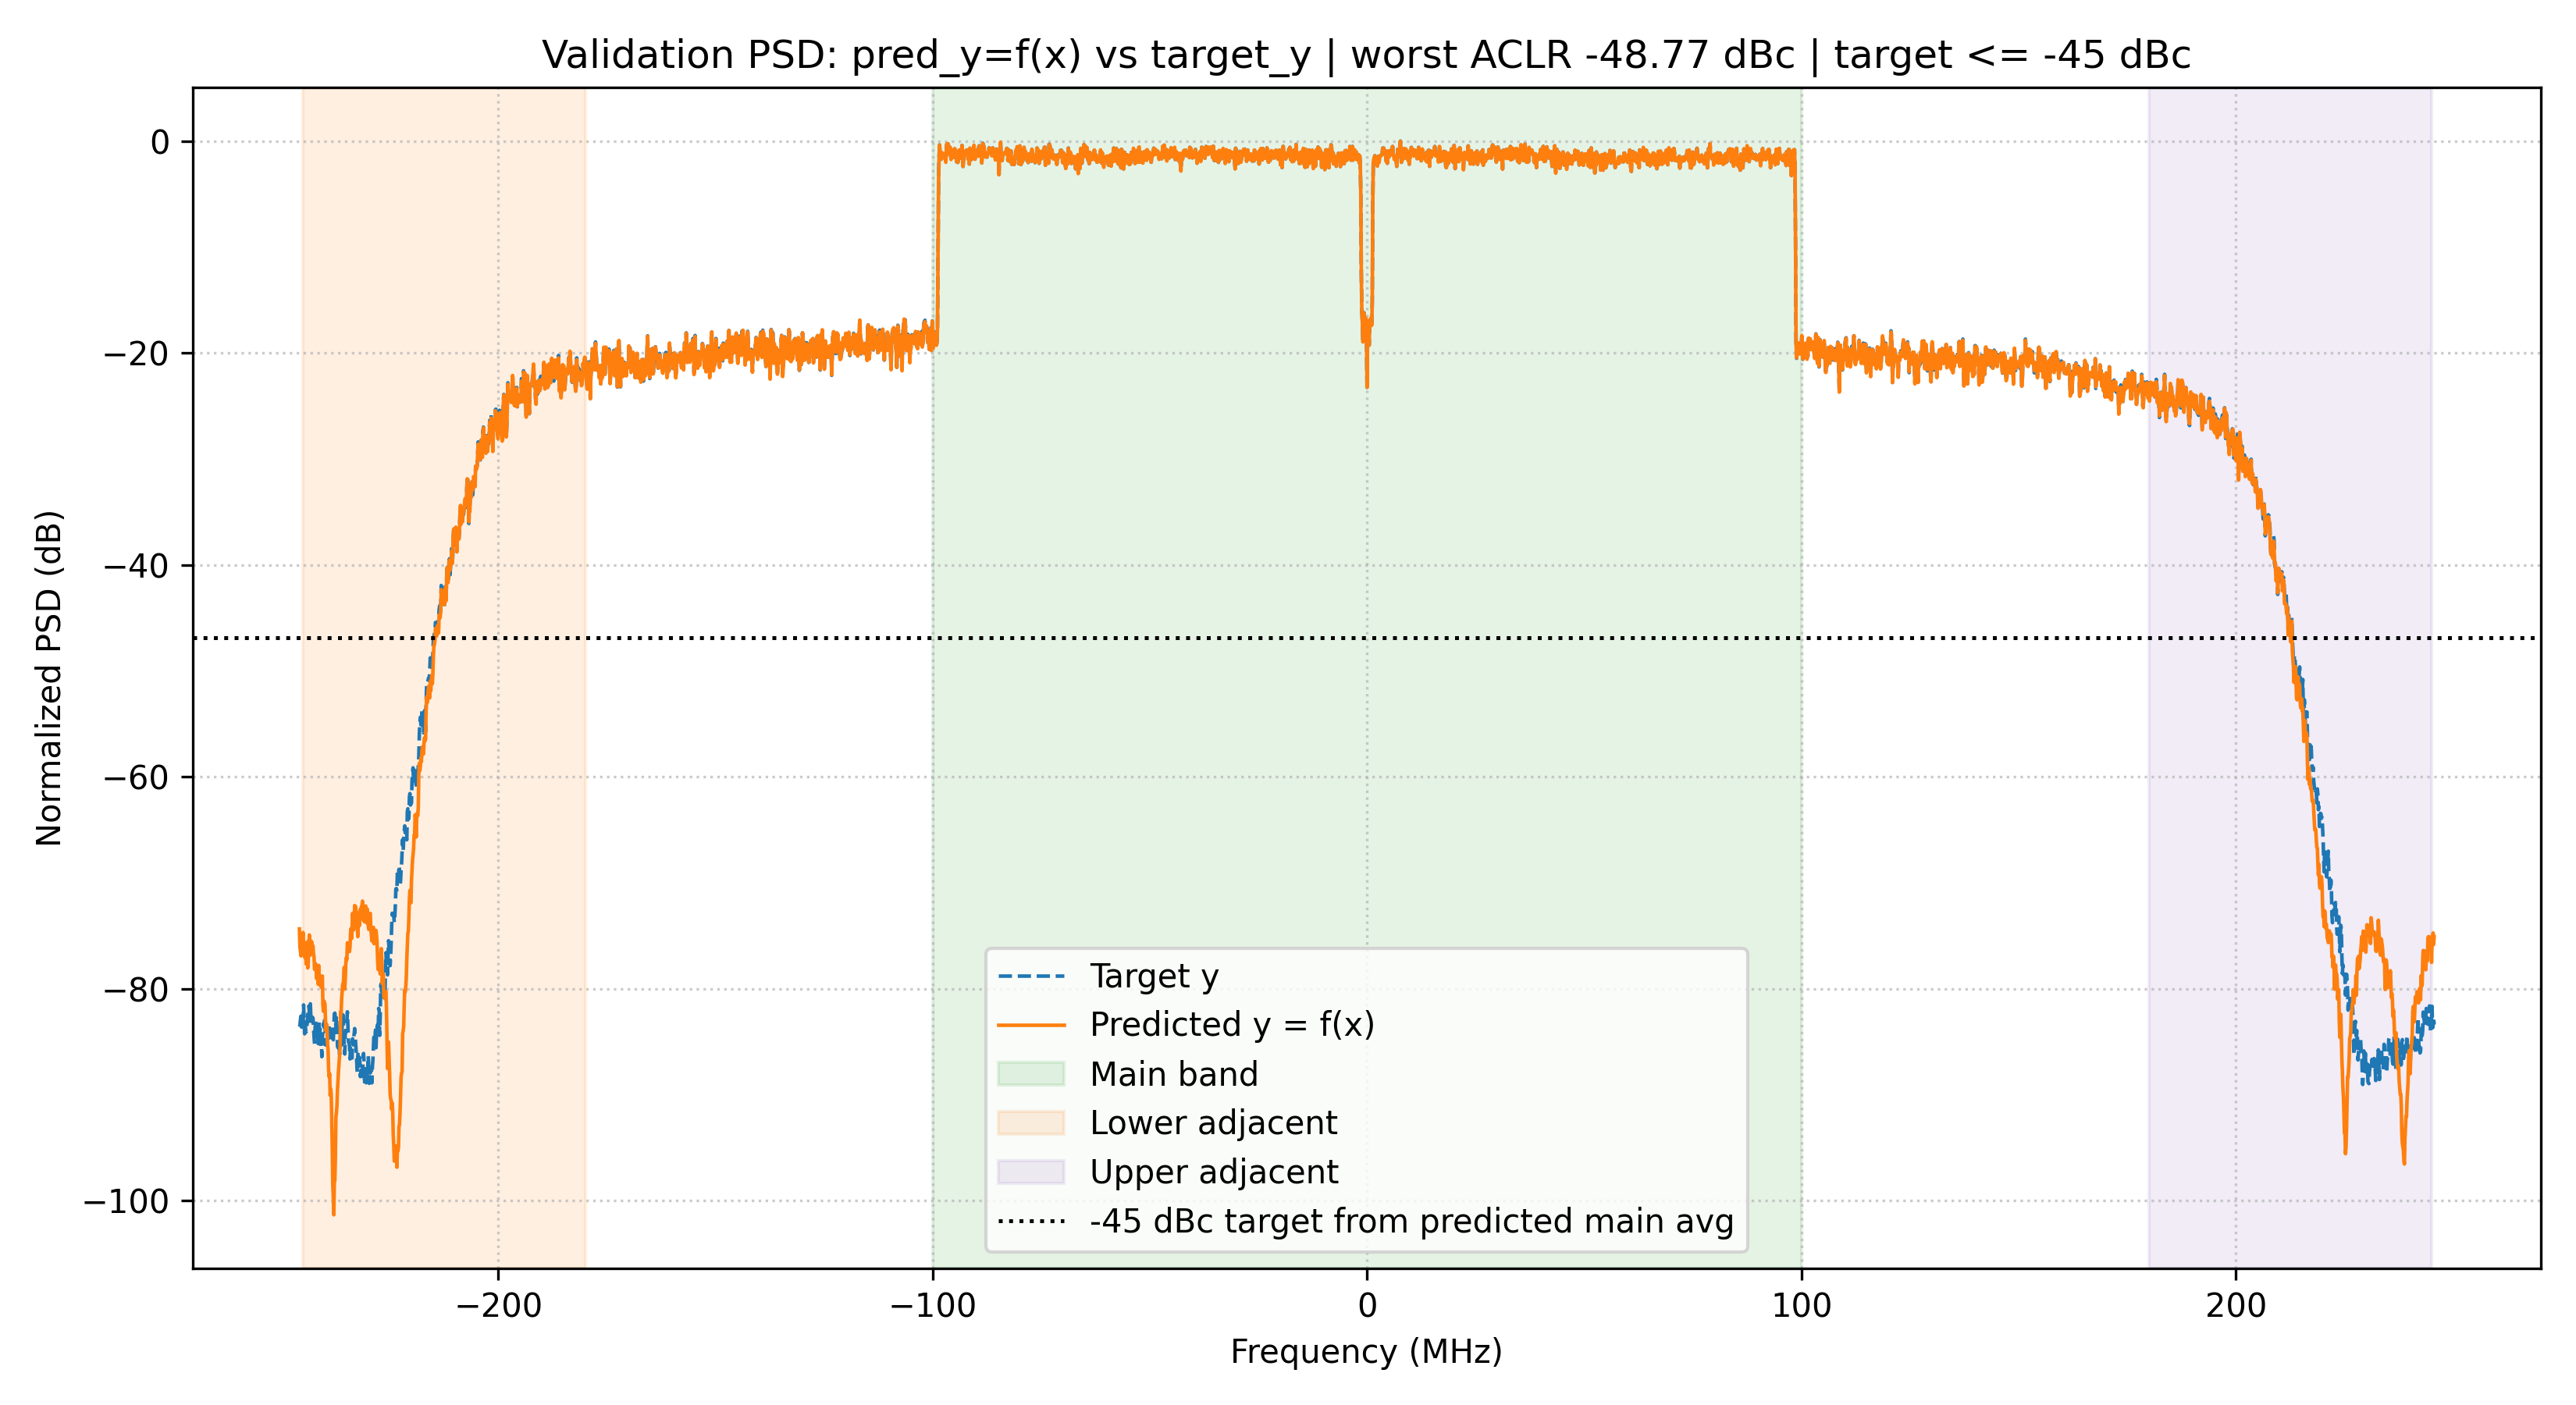
\includegraphics[width=\linewidth]{figures/main_psd_aclr.png}
        \end{column}
        \begin{column}{0.39\linewidth}
          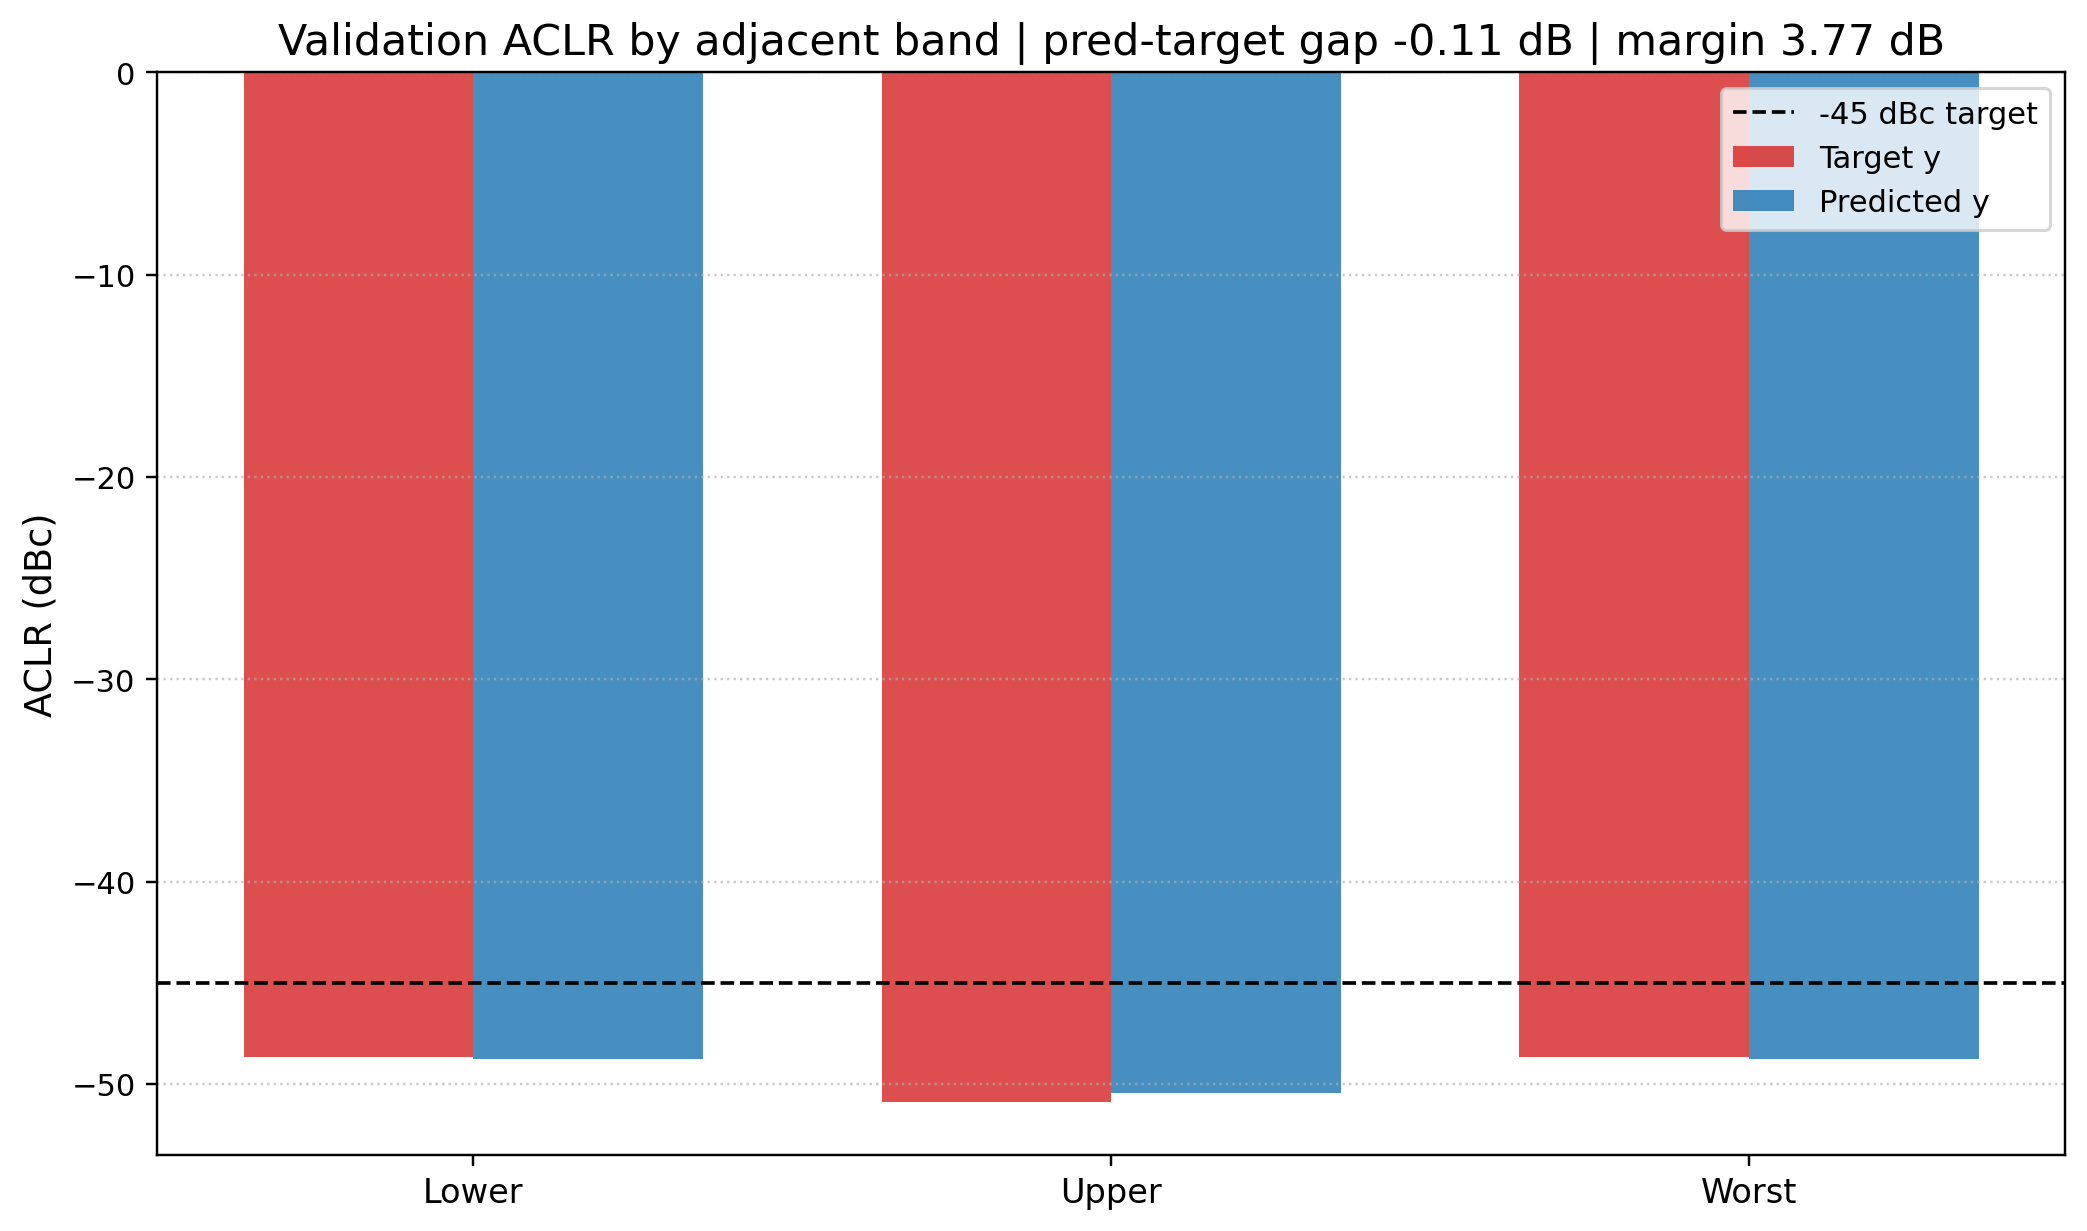
\includegraphics[width=\linewidth]{figures/main_aclr_bar.png}
          \vspace{0.25cm}
          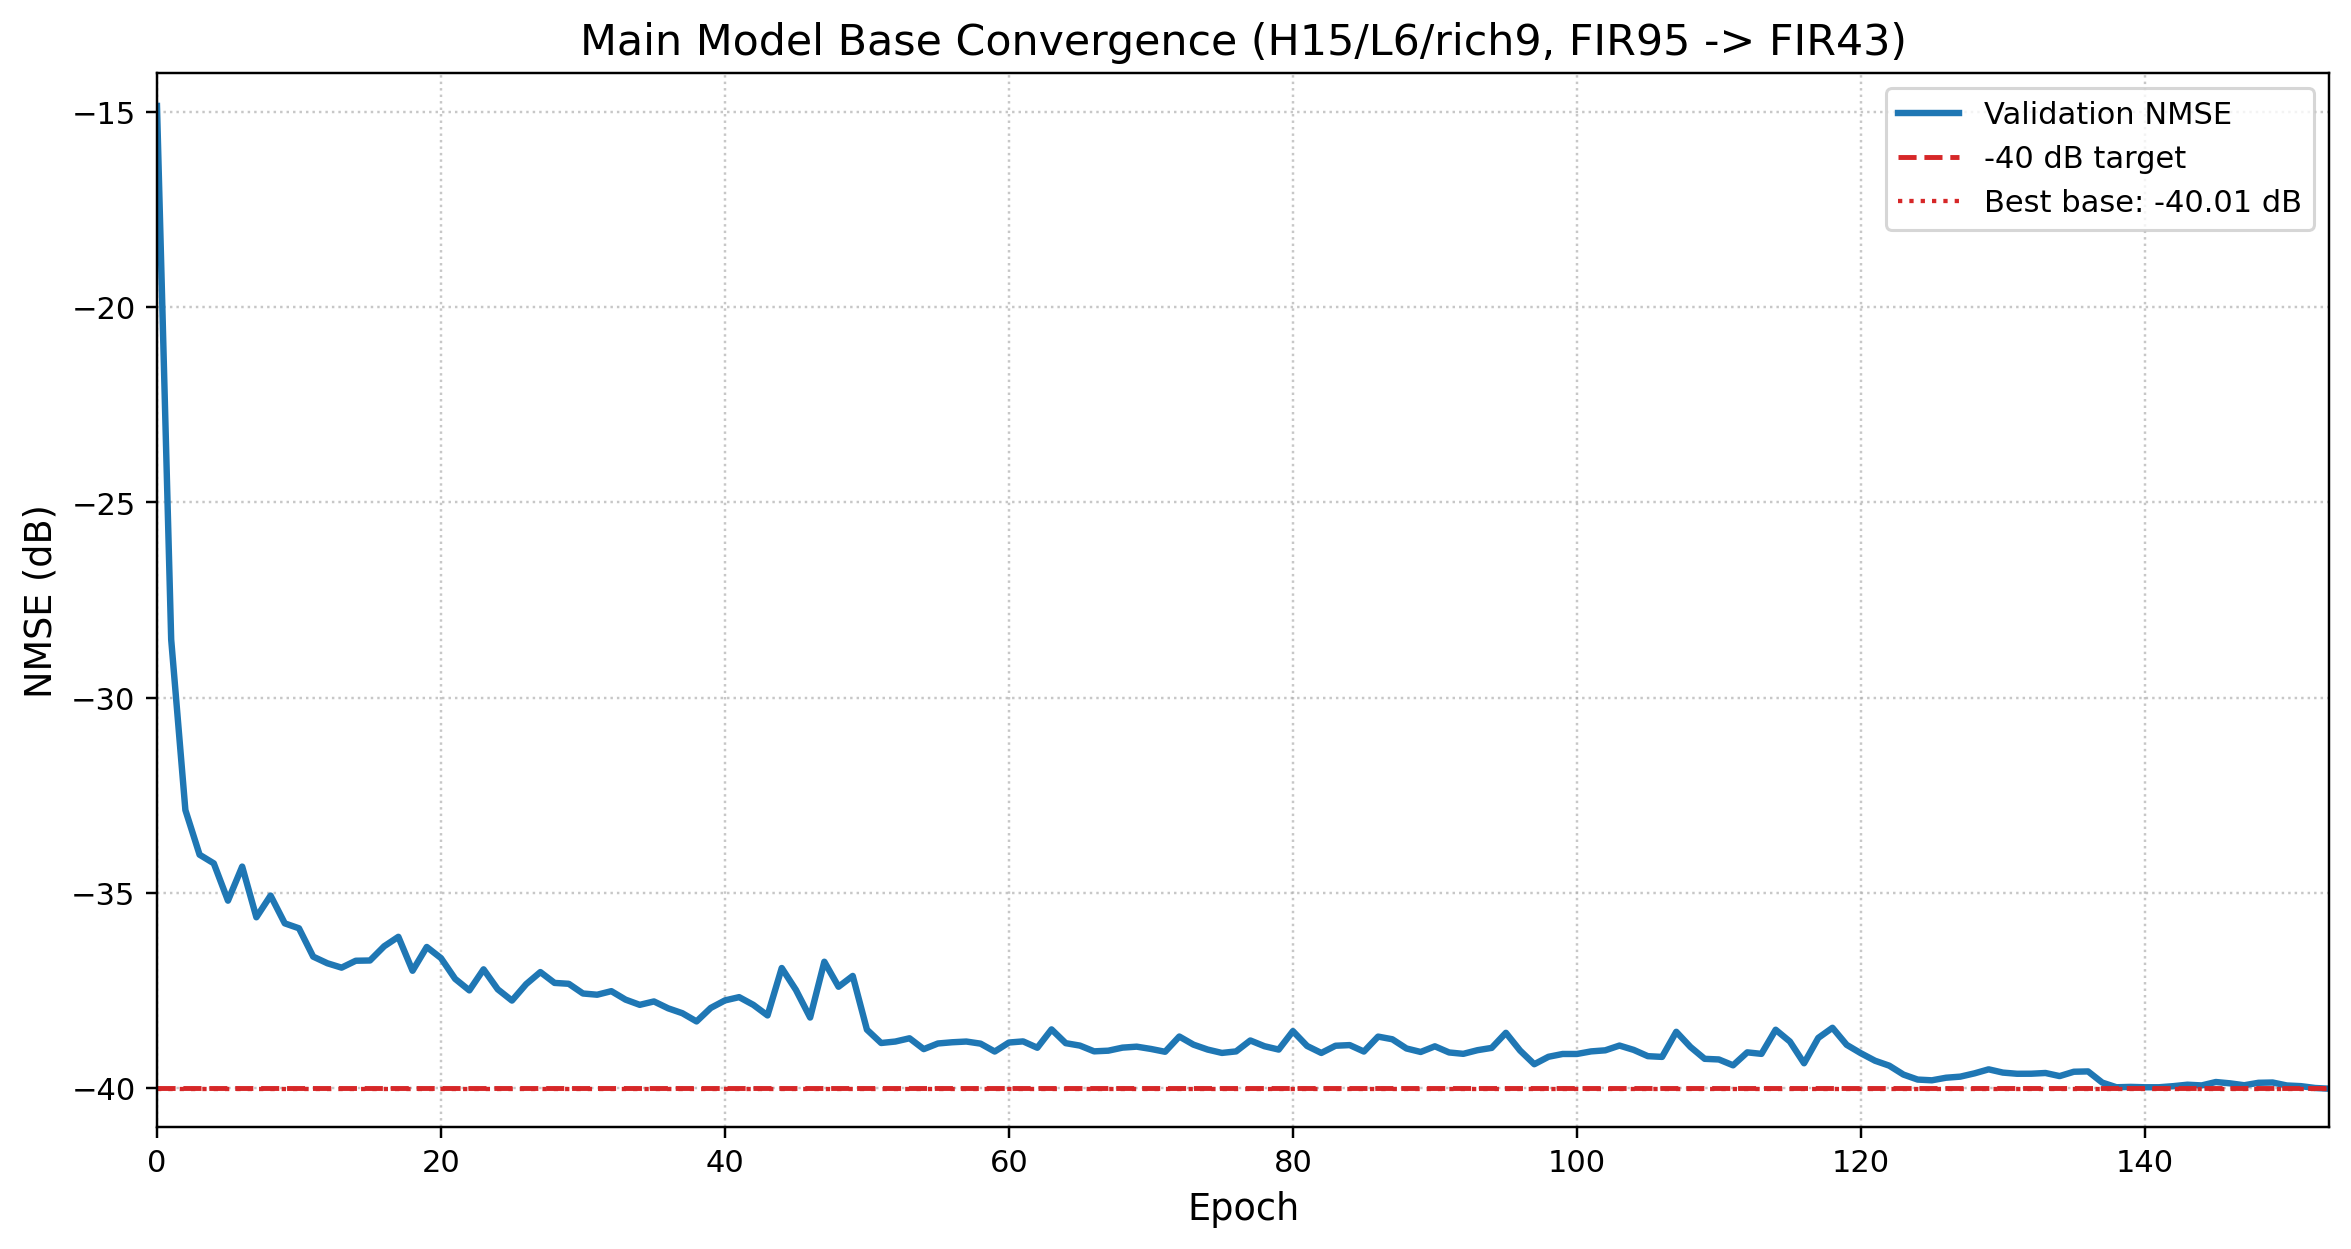
\includegraphics[width=\linewidth]{figures/main_convergence.png}
        \end{column}
      \end{columns}
    \end{column}
  \end{columns}
\end{frame}

\begin{frame}{轻量模型证明 ACLR 可保、NMSE 受主干容量限制}
  \small
  \begin{columns}[T,onlytextwidth]
    \begin{column}{0.48\linewidth}
      \begin{center}
        \textbf{998 MAC：Input-9/attention4/FIR39}\par
        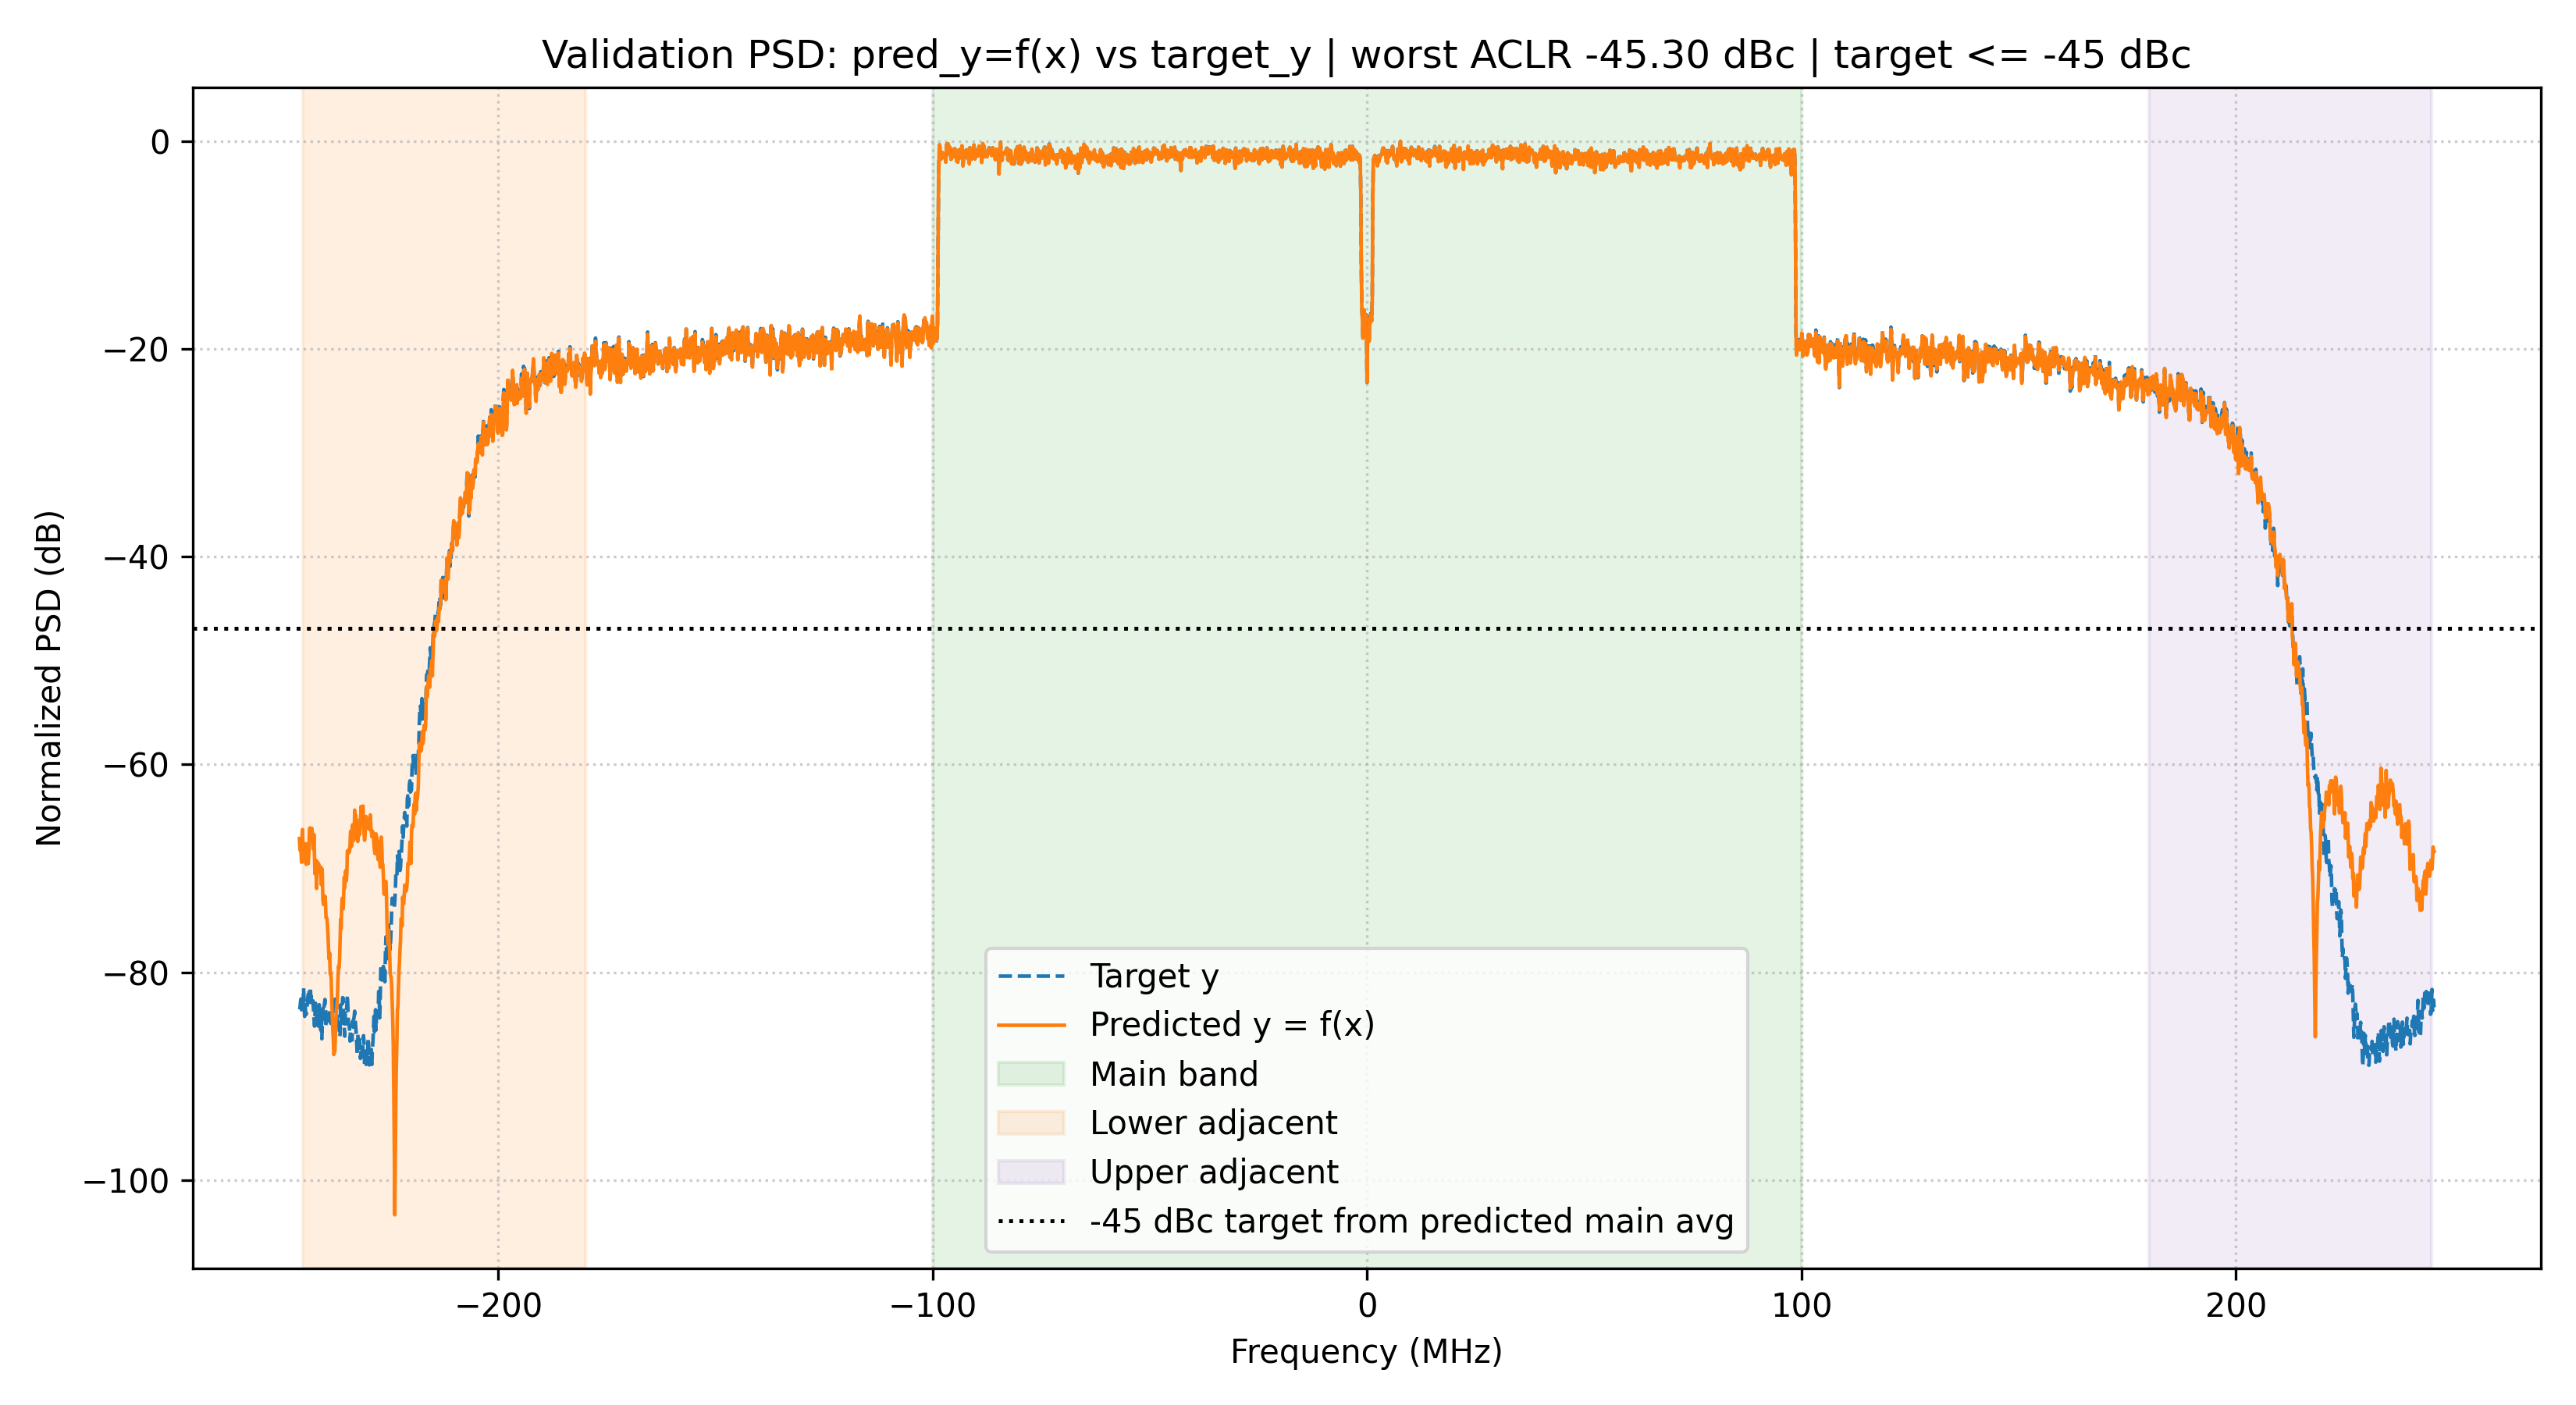
\includegraphics[width=0.82\linewidth]{figures/light998_psd_aclr.png}
      \end{center}
      \metric{metricwarn}{NMSE -37.37 dB}{ACLR -45.30 dBc；ACLR 达标，NMSE 未达标}
    \end{column}
    \begin{column}{0.48\linewidth}
      \begin{center}
        \textbf{796 MAC：H10/L3/Input-6/FIR41}\par
        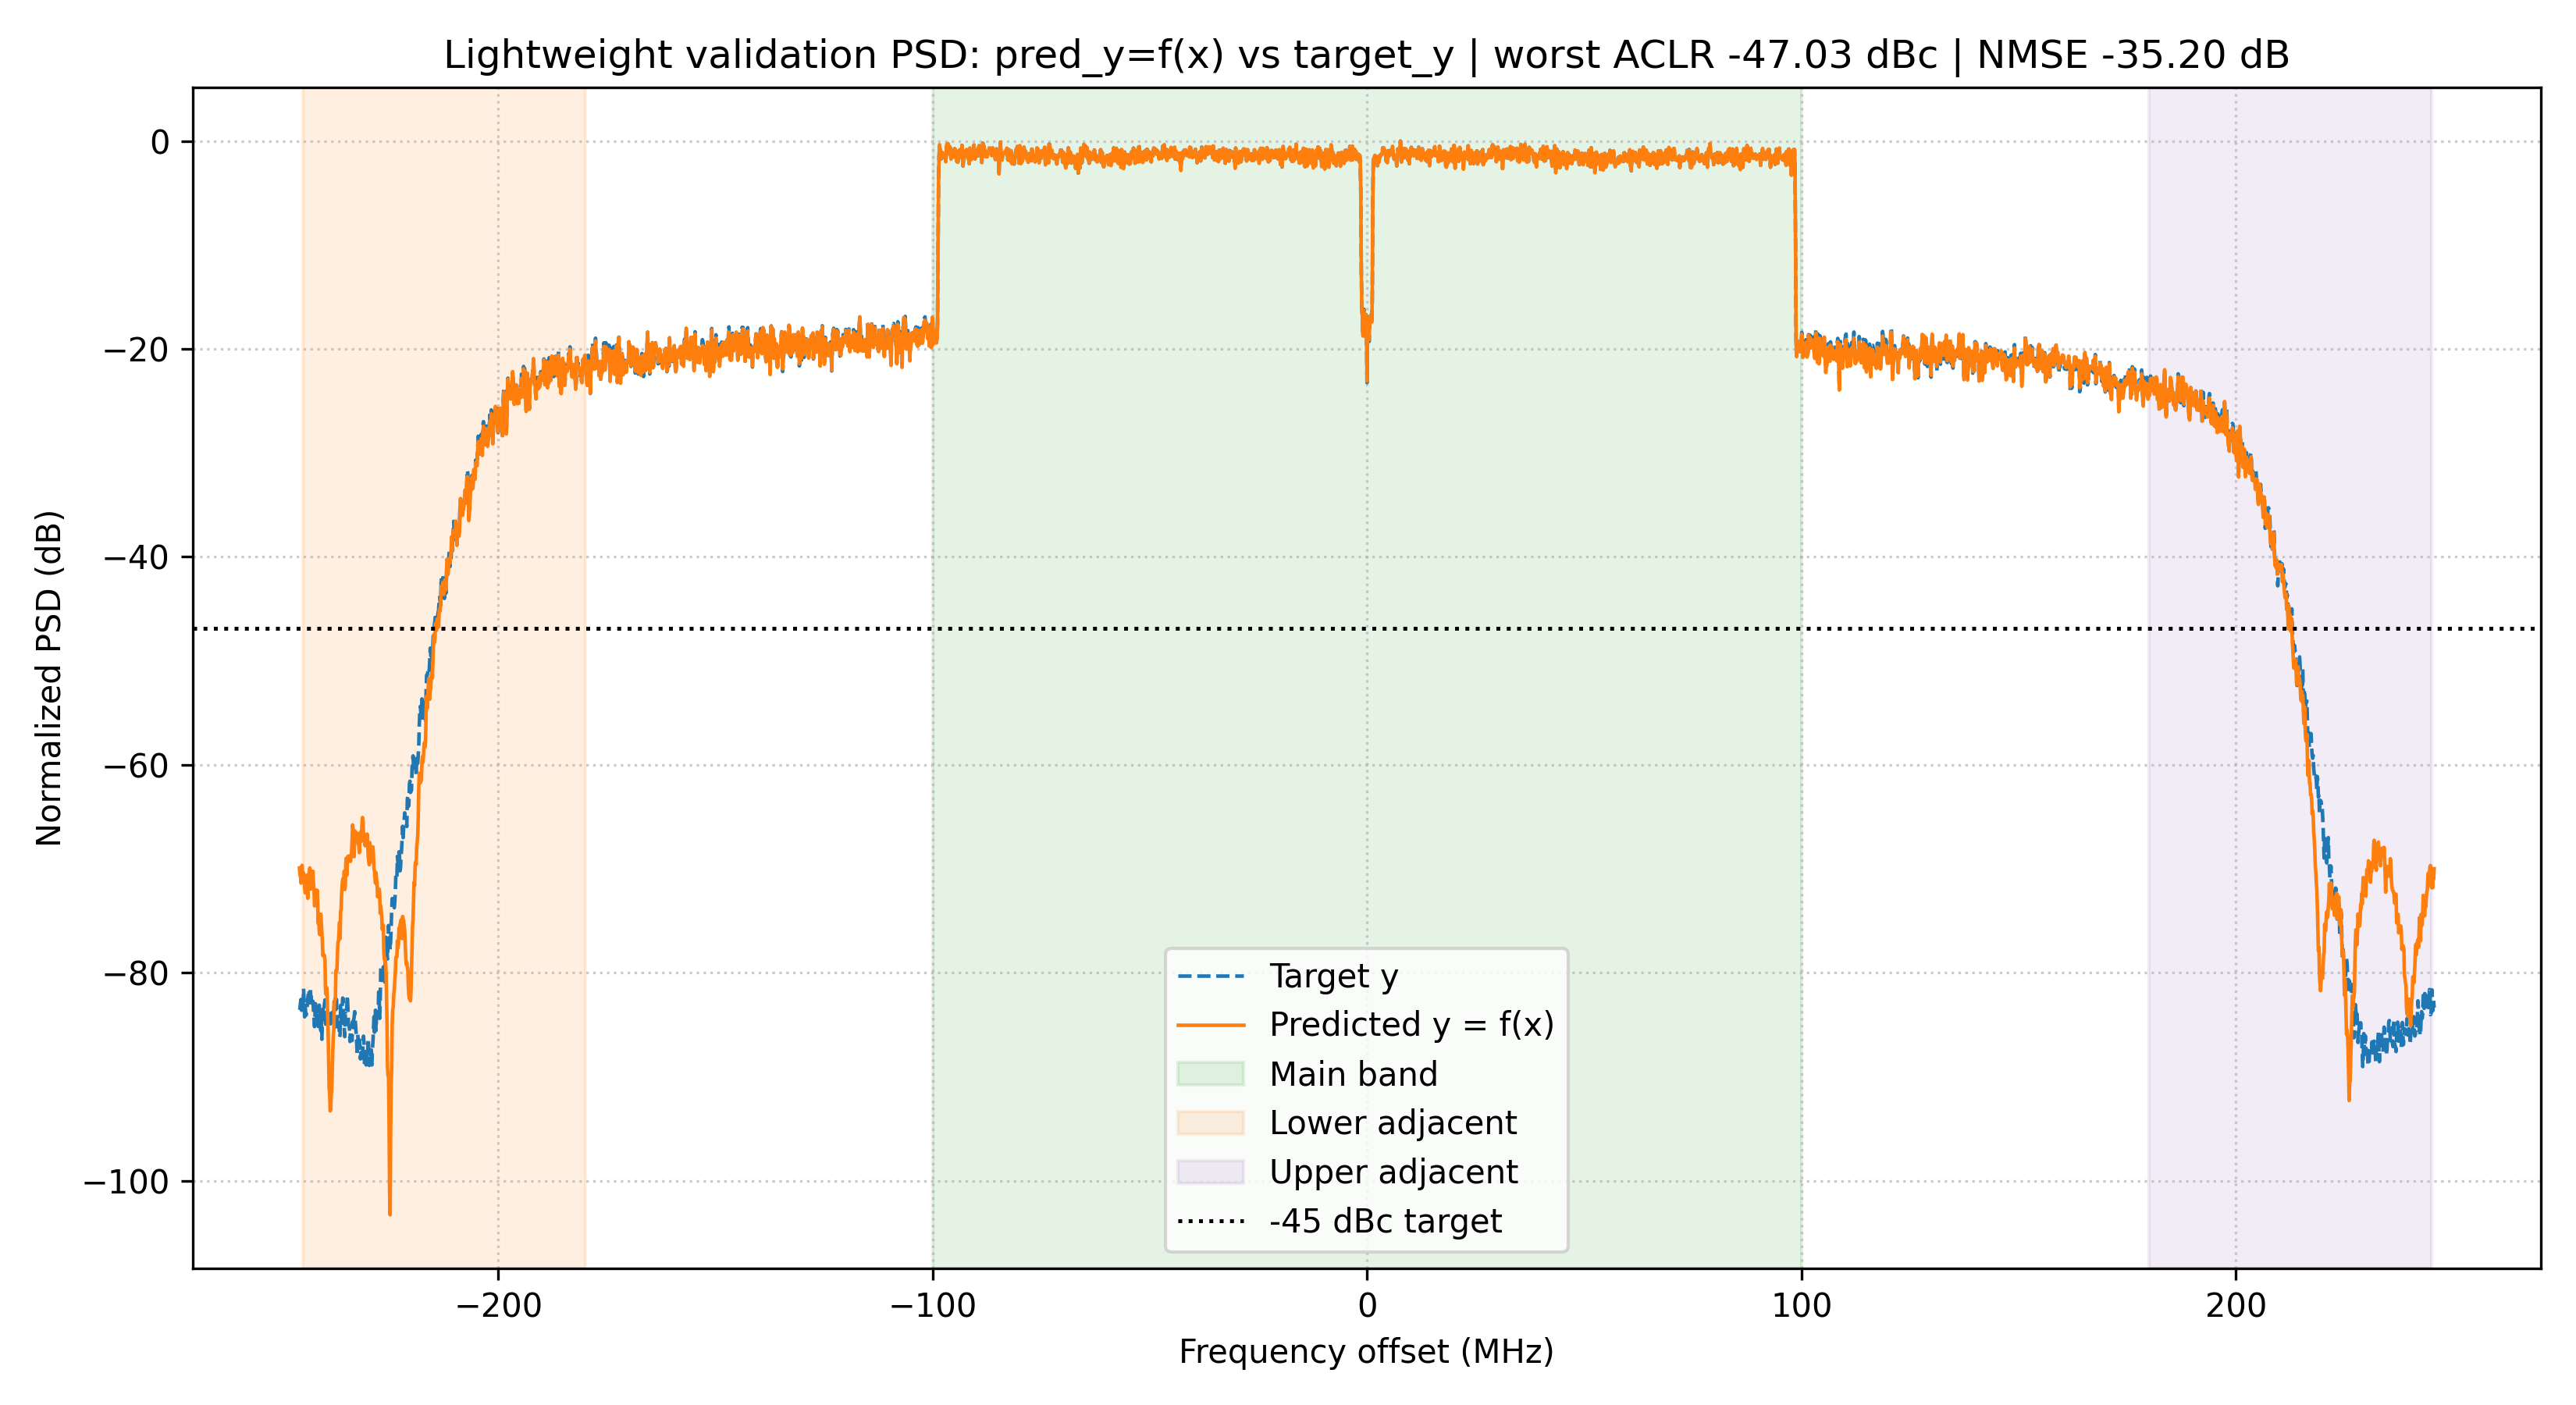
\includegraphics[width=0.82\linewidth]{figures/light796_psd_aclr.png}
      \end{center}
      \metric{metricwarn}{NMSE -35.20 dB}{ACLR -47.03 dBc；ACLR 达标，NMSE 未达标}
    \end{column}
  \end{columns}

  \vspace{0.25cm}
  \begin{beamercolorbox}[wd=\linewidth,sep=0.55em]{card}
    结论：FIR 与频域校正能守住邻道泄漏，但极低 MAC 下的 TCN 主干容量成为 NMSE 的主要瓶颈。
  \end{beamercolorbox}
\end{frame}

\begin{frame}{786 MAC 低复杂度模型专项结果}
  \small
  \begin{columns}[T,onlytextwidth]
    \begin{column}{0.47\linewidth}
      \begin{beamercolorbox}[wd=\linewidth,sep=0.5em]{metricblue}
        \textbf{结构卡片}\par
        H10/L4/Input-6/pointwise rank 3/FIR41\par
        \textbf{786 real multipliers}\par
        {\scriptsize checkpoint: \path{step800_scratch_h10_l4_base6_rank3_fir41_786.pth}}
      \end{beamercolorbox}
      \vspace{0.12cm}
      {\scriptsize
      variant / preset: \code{h10_l4_base6_rank3_fir41} / \code{h10_l4_base6_rank3_fir41_786}\par
      prefix: \code{step800_scratch_h10_l4_base6_rank3_fir41_786}\par
      dilations: $[1,2,4,8]$；attention channels: 3；poly orders: $[1,3,5]$
      }
    \end{column}
    \begin{column}{0.49\linewidth}
      \begin{columns}[T,totalwidth=\linewidth]
        \begin{column}{0.49\linewidth}
          \metric{metricwarn}{NMSE -35.46 dB}{距 -40 dB 约 4.54 dB}
        \end{column}
        \begin{column}{0.49\linewidth}
          \metric{metricpass}{worst ACLR -46.76 dBc}{相对门限约 1.76 dB 余量}
        \end{column}
      \end{columns}
      \vspace{0.3cm}
      \begin{beamercolorbox}[wd=\linewidth,sep=0.45em]{card}
        Linear NMSE: $2.8431769286770583\times10^{-4}$；lower ACLR: -46.76 dBc；upper ACLR: -48.40 dBc。
      \end{beamercolorbox}
    \end{column}
  \end{columns}

  \vspace{0.2cm}
  \begin{columns}[T,onlytextwidth]
    \begin{column}{0.39\linewidth}
      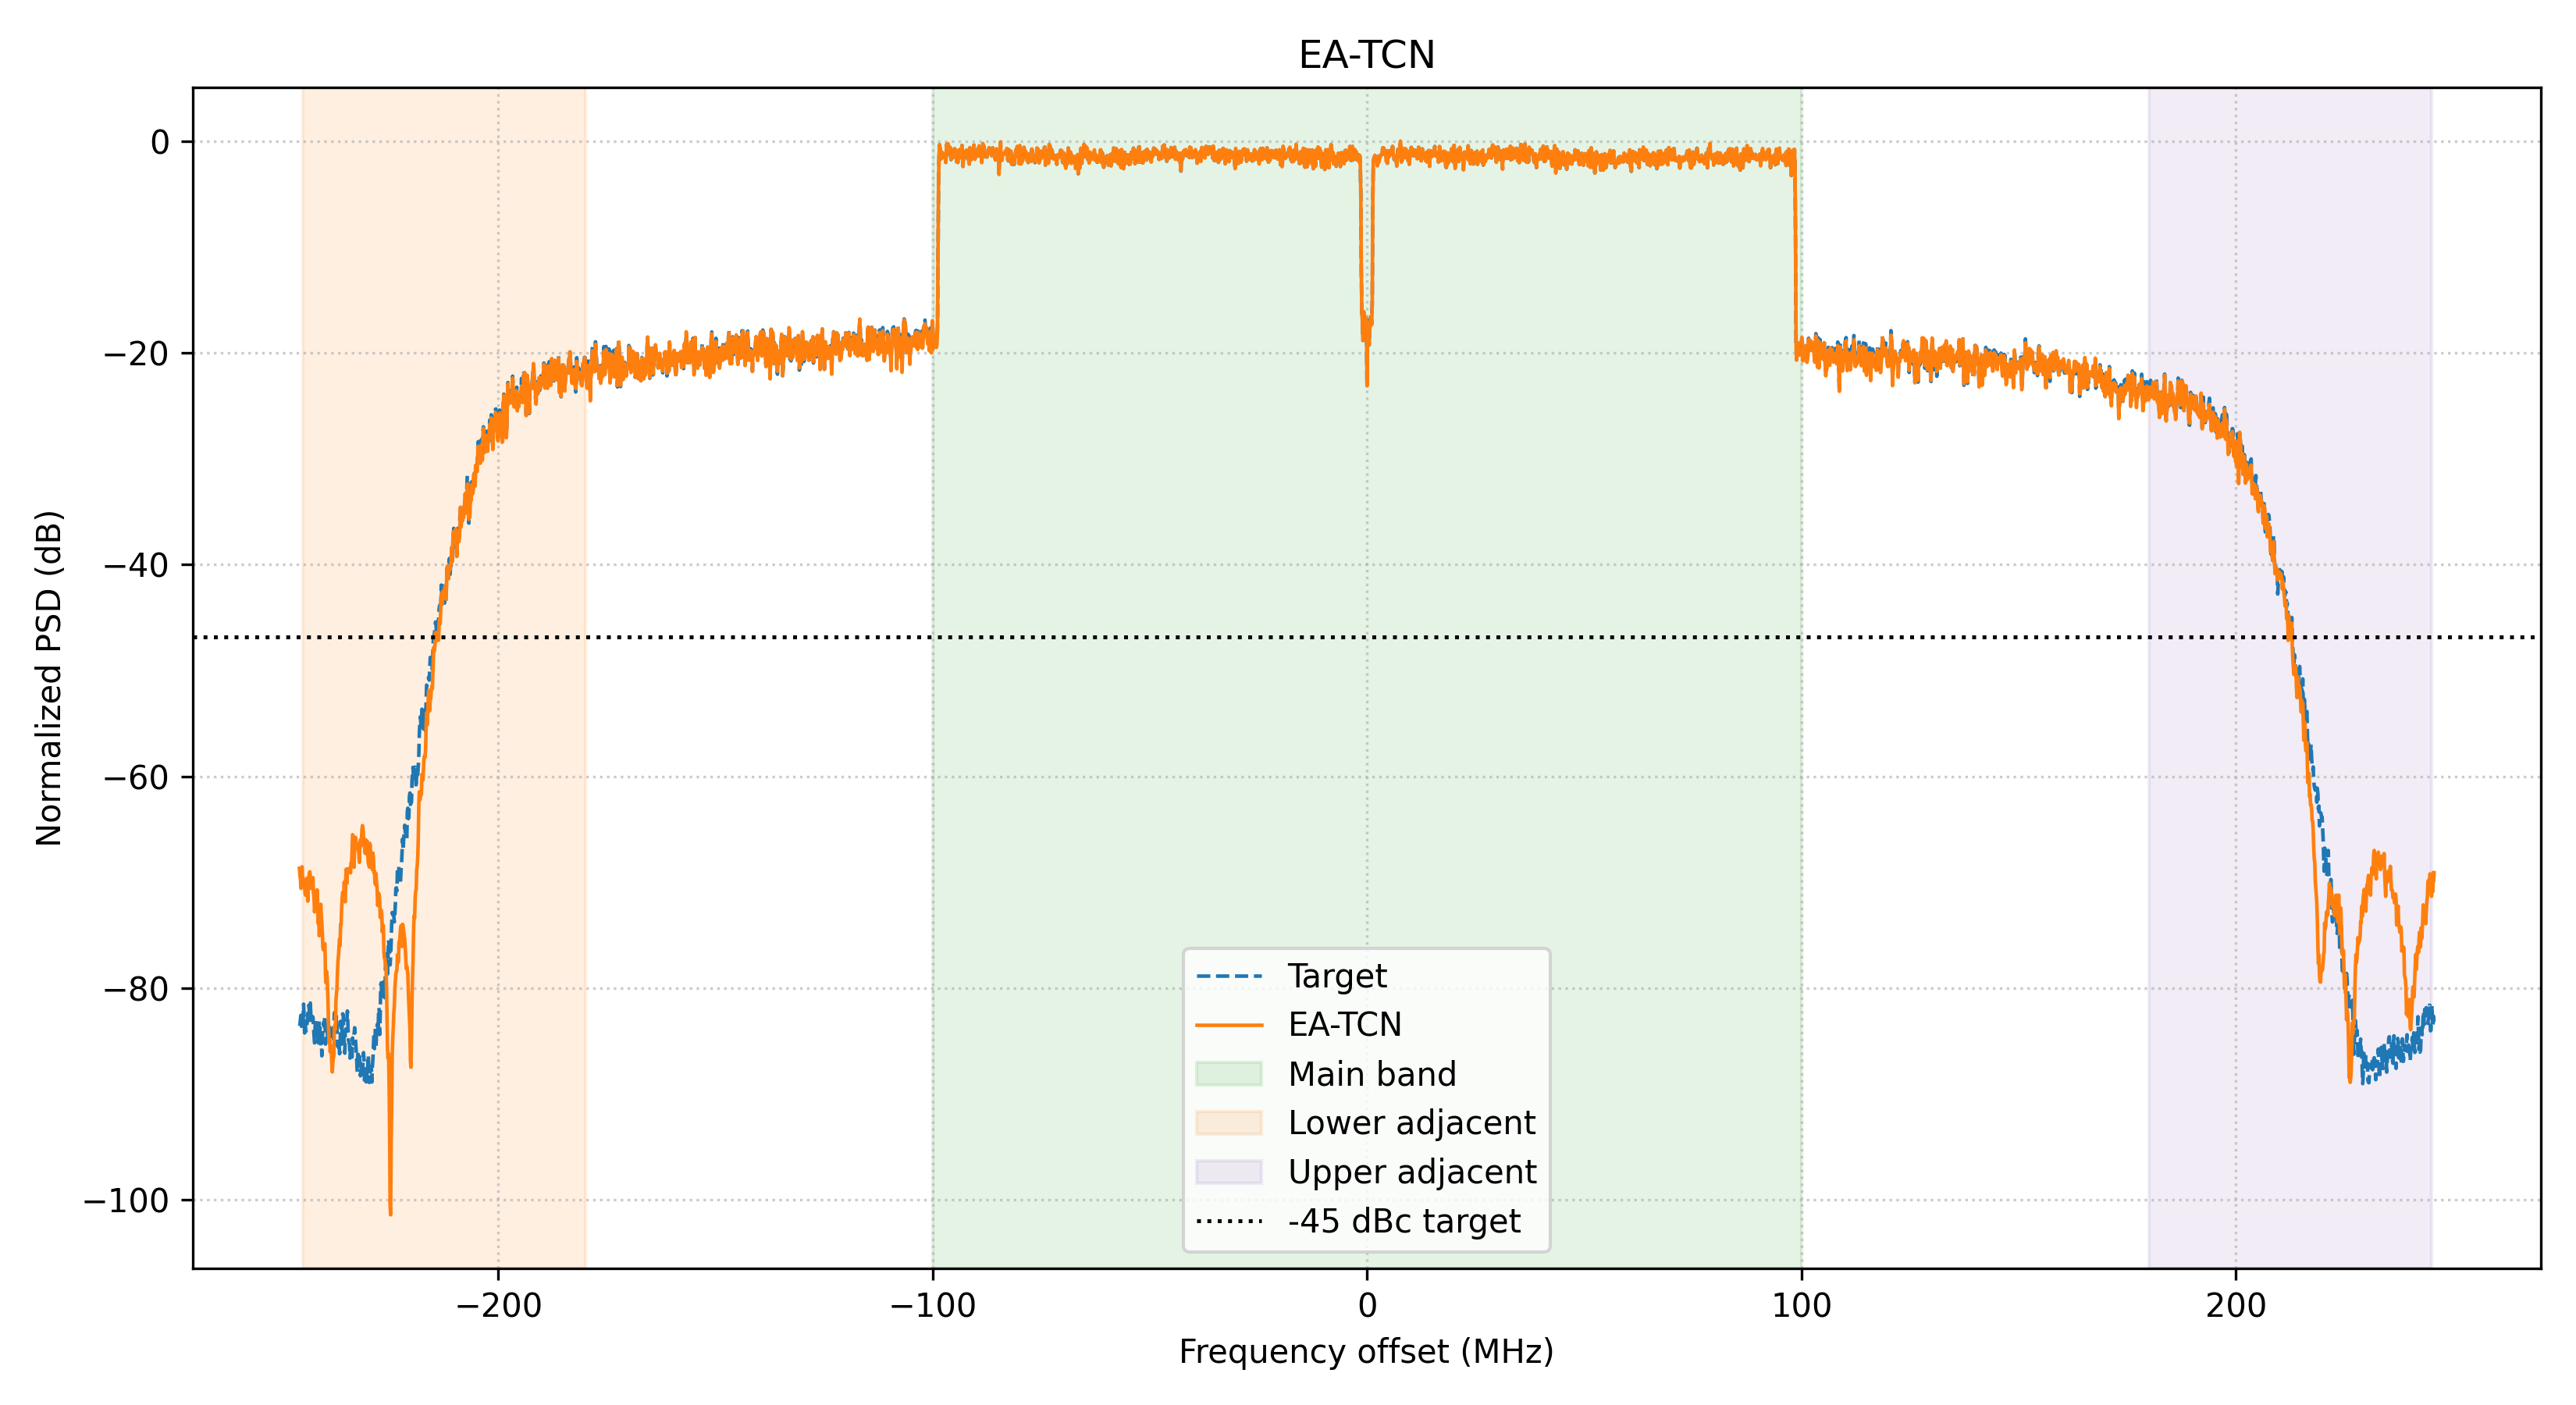
\includegraphics[width=\linewidth,height=3.85cm,keepaspectratio]{figures/model786_psd_aclr.png}
    \end{column}
    \begin{column}{0.23\linewidth}
      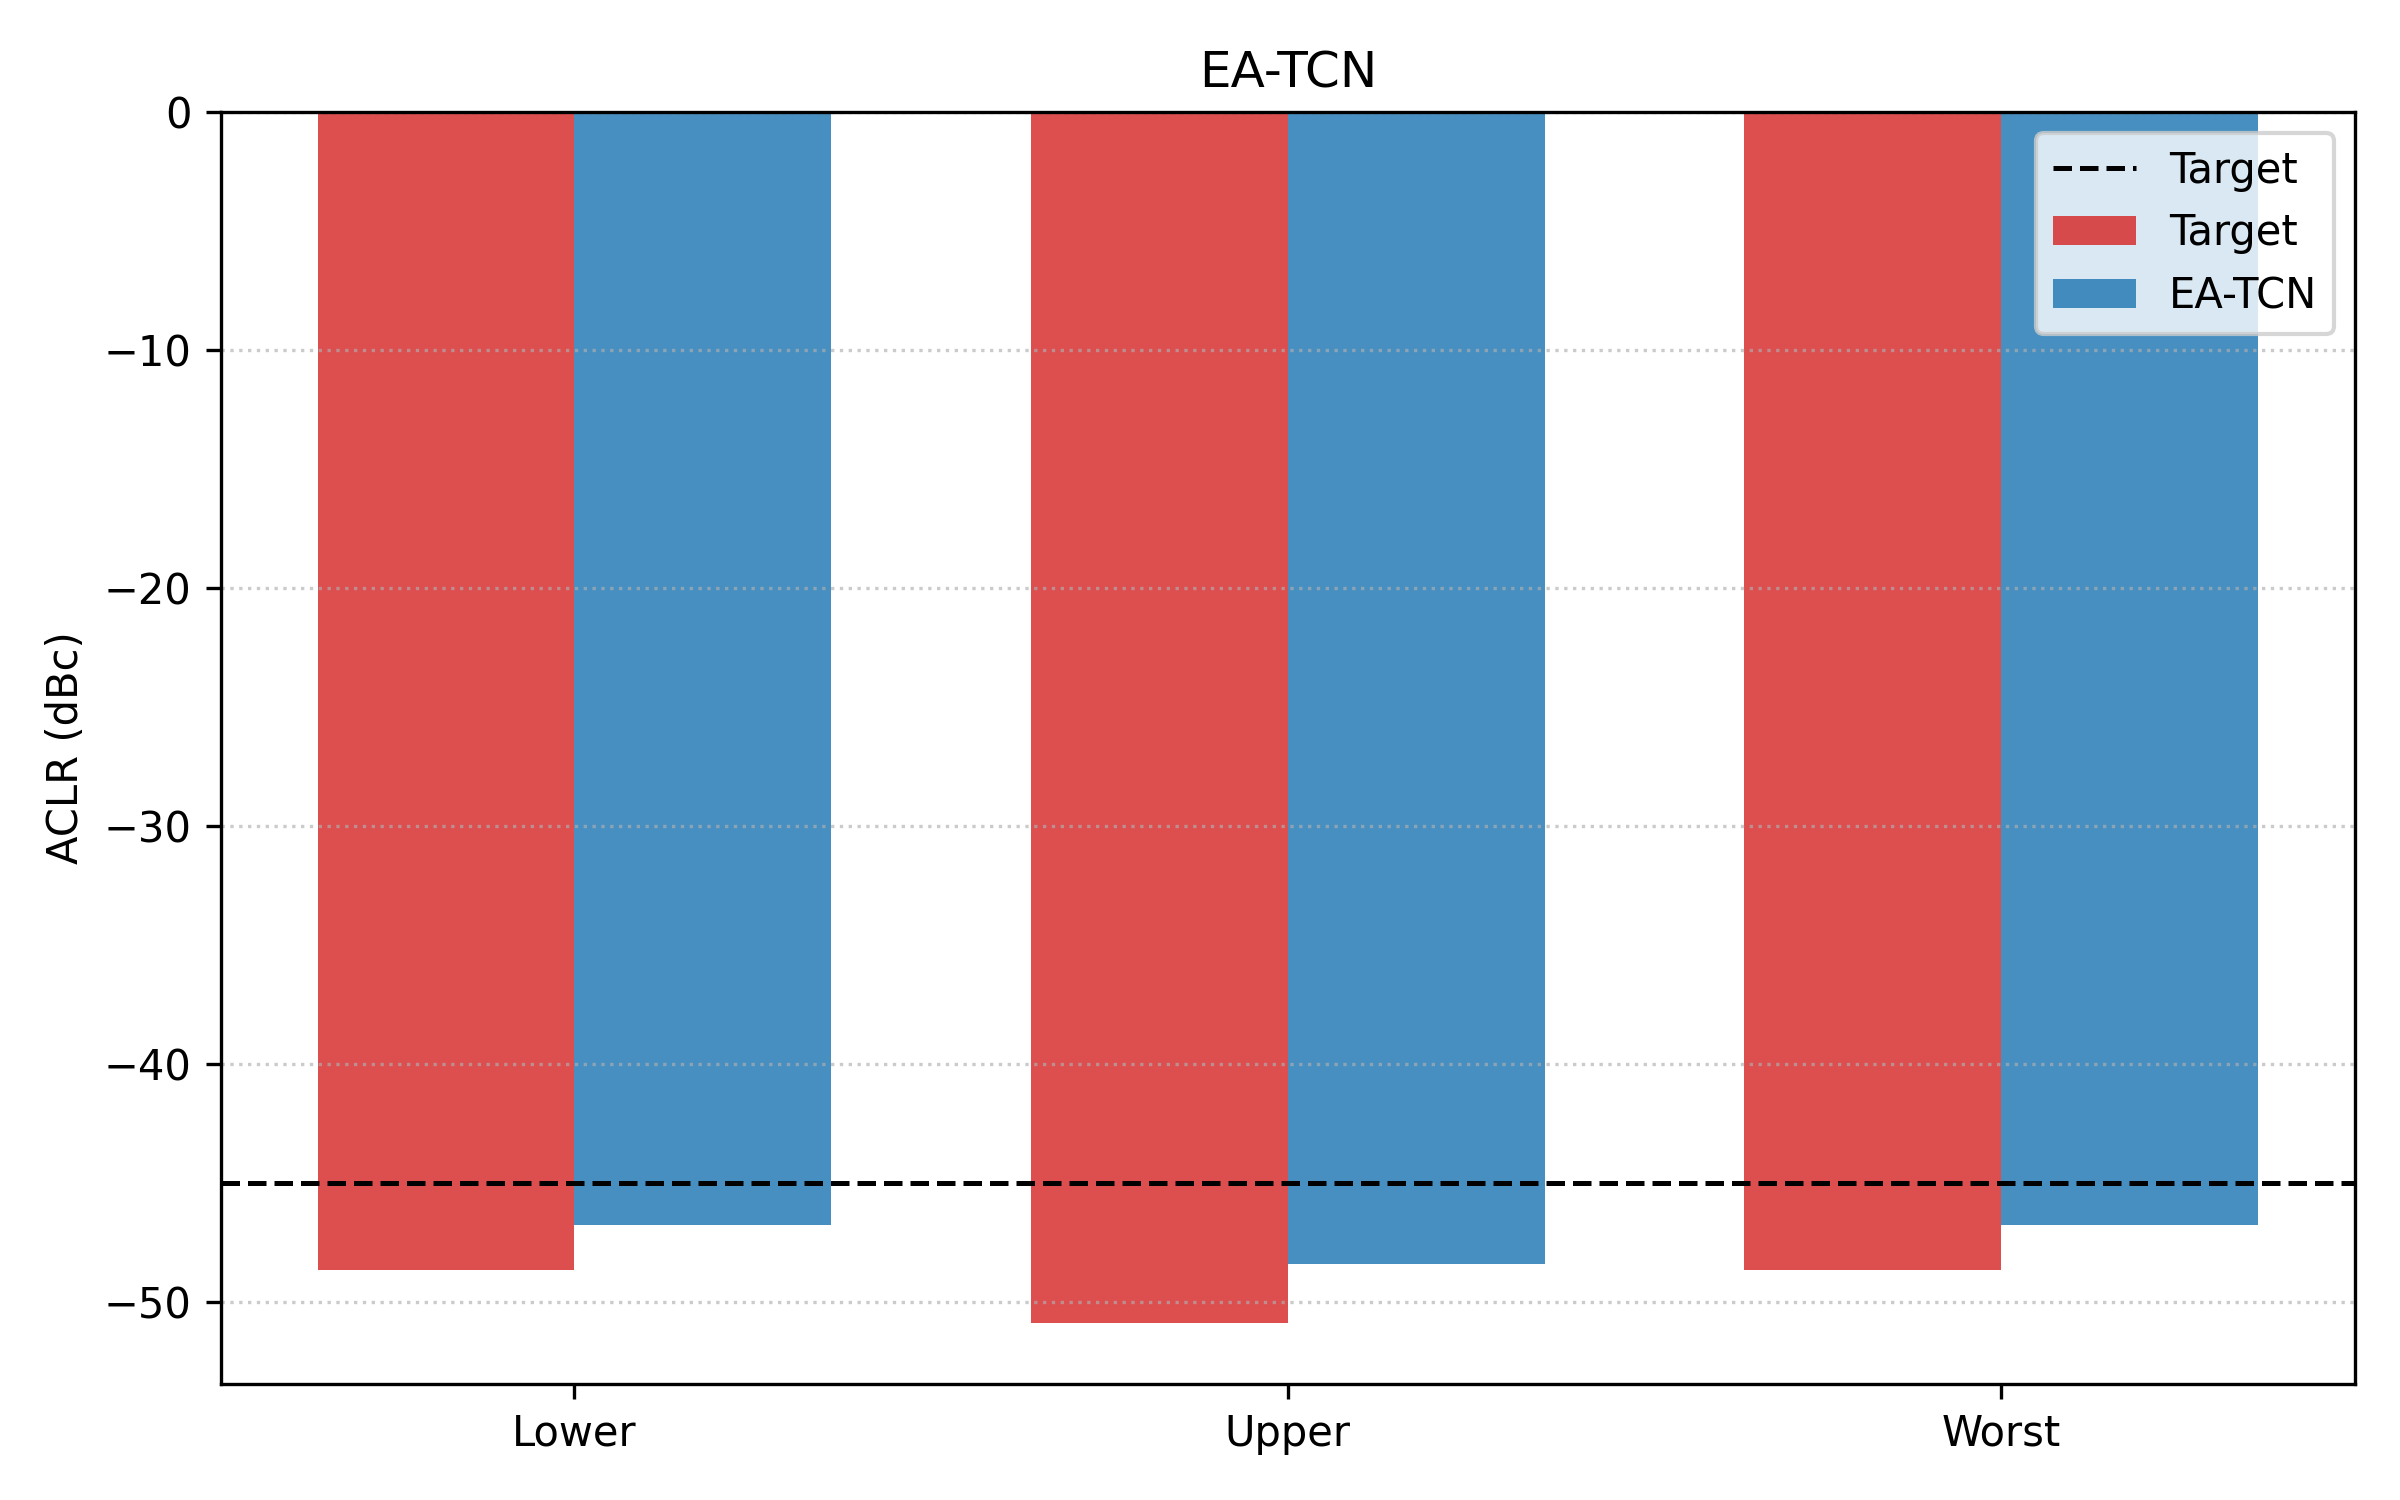
\includegraphics[width=\linewidth,height=1.82cm,keepaspectratio]{figures/model786_aclr_bar.png}
      \vspace{0.06cm}
      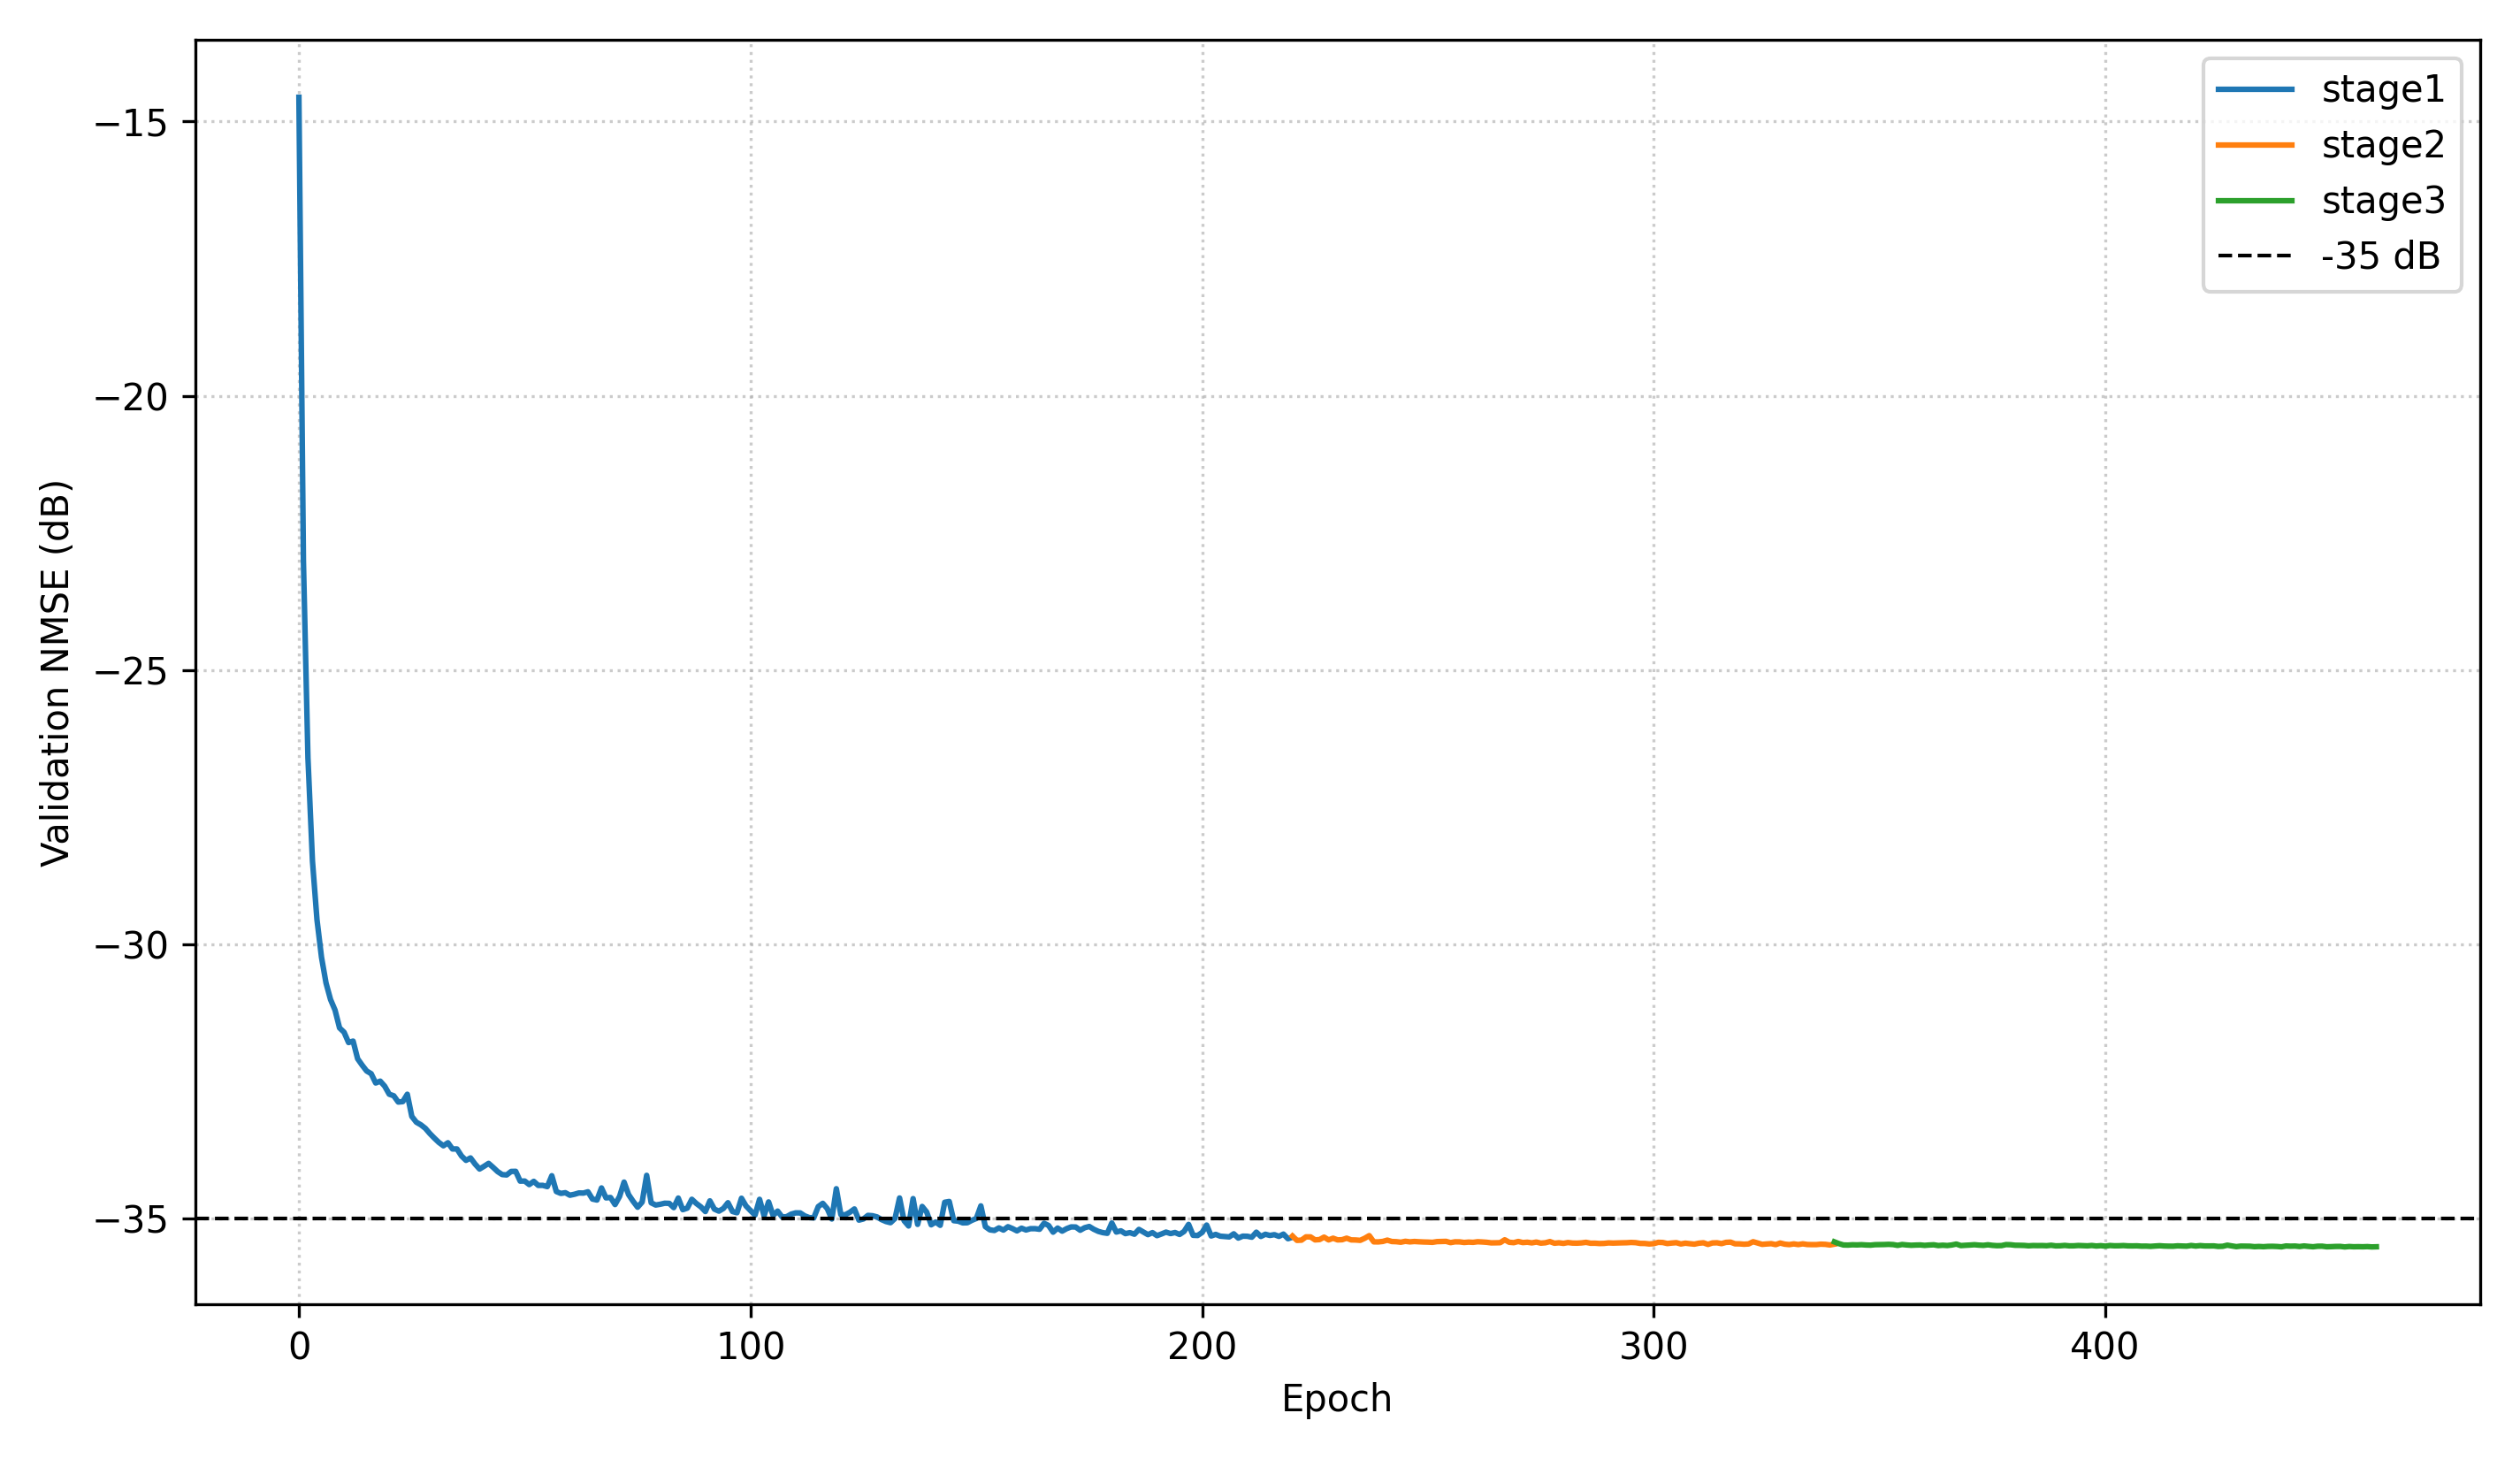
\includegraphics[width=\linewidth,height=1.82cm,keepaspectratio]{figures/model786_convergence.png}
    \end{column}
    \begin{column}{0.34\linewidth}
      \scriptsize
      \begin{itemize}
        \item FIR41 保住邻道泄漏，ACLR 有约 1.76 dB 余量。
        \item L4 + rank3 pointwise 接近 796 baseline，但主干容量不足。
        \item $\le 800$ MAC 的主要瓶颈是非线性拟合能力，不是频域校正。
      \end{itemize}
    \end{column}
  \end{columns}
\end{frame}

\section{结论}
\begin{frame}{结题结论与后续工作}
  \begin{columns}[T,onlytextwidth]
    \begin{column}{0.48\linewidth}
      \begin{beamercolorbox}[wd=\linewidth,sep=0.85em]{metricpass}
        \textbf{已完成目标}\par
        EA-TCN 主模型在 2284 个等效实数乘法器下达到 NMSE -40.15 dB 与 worst ACLR -48.77 dBc，满足赛题双指标。
      \end{beamercolorbox}

      \vspace{0.45cm}
      \begin{beamercolorbox}[wd=\linewidth,sep=0.85em]{metricwarn}
        \textbf{轻量化边界}\par
        998、796、786 MAC 模型均能保持 ACLR 达标，但 NMSE 未达标，说明极低复杂度下主干容量是关键限制。
      \end{beamercolorbox}
    \end{column}
    \begin{column}{0.48\linewidth}
      \begin{itemize}
        \item 从 2284/2268 MAC 达标模型出发做结构化剪枝。
        \item 对 pointwise 混合层继续做低秩分解与恢复训练。
        \item 引入 QAT 定点量化，评估 FPGA/DSP 流水实现。
        \item 保留频域带权 refit，持续约束邻道泄漏。
      \end{itemize}

      \vspace{0.55cm}
      \begin{center}
        {\Large\textcolor{cquptblue}{谢谢各位老师指导}}
      \end{center}
    \end{column}
  \end{columns}
\end{frame}

\end{document}
